\documentclass{sig-alt-full}
\usepackage{graphics}
\usepackage{hhline}
\usepackage{alltt}
\usepackage{url}
%\usepackage{times}
\usepackage{xspace}
\usepackage{cite}

%% The name of the system is....?
\def\Sys{P2\xspace}
\def\Lang{OverLog\xspace}
\def\ELang{PEL\xspace}
\def\Elang{\ELang}
\def\PChordLines{47\xspace}
\def\MacChordLines{320\xspace}
\def\PNaradaLines{16\xspace}

\newcommand{\ol}[1]{{\tt\footnotesize#1}}
\newenvironment{overlog}{\begin{alltt}\small}{\end{alltt}}

\newcommand{\note}[1]{}

\begin{document}
\conferenceinfo{SOSP'05,} {October 23--26, 2005, Brighton, United Kingdom.}
\CopyrightYear{2005}
\crdata{1-59593-079-5/05/0010}
\bibliographystyle{abbrv}
\title{Implementing Declarative Overlays}


\numberofauthors{3}
\author{
\alignauthor
Boon Thau Loo\thanks{Boon Thau Loo and Tyson Condie are supported in
  part by the National Science Foundation under Grants No.\ 0205647,
  0209108, and 0225660, and by a gift from Microsoft Corporation.}\\
{\affaddr UC Berkeley}\\
\vspace{24pt}
Petros Maniatis\\
{\affaddr Intel Research Berkeley}
\alignauthor
Tyson Condie$^*$\\
{\affaddr UC Berkeley}\\
\vspace{24pt}
Timothy Roscoe\\
{\affaddr Intel Research Berkeley}
\alignauthor
Joseph M.\ Hellerstein\\
{\affaddr Intel Research Berkeley}\\
{\affaddr UC Berkeley}\\
\vspace{13.5pt}
Ion Stoica\\
{\affaddr UC Berkeley}
}
\date{}
\maketitle
%\thispagestyle{plain}

%% {\footnotesize
%% \begin{verbatim}
%% $Id: camready.tex,v 1.19 2005/08/13 17:37:34 troscoe Exp $
%% \end{verbatim}
%% }
\begin{abstract}
Overlay networks are used today in a variety of distributed systems
ranging from file-sharing and storage systems to communication
infrastructures.  However, designing, building and adapting these
overlays to the intended application and the target environment is a
difficult and time consuming process.

To ease the development and the deployment of such overlay networks
we have implemented \Sys, a system that uses a declarative logic
language to express overlay networks in a highly compact and
reusable form. \Sys can express a Narada-style mesh network in
\PNaradaLines rules, and the Chord structured overlay in only
\PChordLines rules.  \Sys directly parses and executes such
specifications using a dataflow architecture to construct and maintain
overlay networks.  We describe the \Sys approach, how our
implementation works, and show by experiment its promising trade-off point
between specification complexity and performance.

\end{abstract}

\category{C.2.4}{Computer Communication Networks}{Distributed
  Systems}[distributed applications]
\category{D.4.7}{Operating Systems}{Organization
  and Design}[Distributed systems]
\category{C.2.2}{Computer Communication Networks}{Network
  Protocols}[protocol architecture, routing protocols]


\terms{Design, Experimentation, Languages}

\keywords{Declarative overlays, dataflow engines, executable pseudocode}



% % % % % % % % % % % % % % % % % % % % % % % % % % % % % % % % % % 
\section{Introduction}
\label{sec:intro}
\note{Motivation: relevance.}
Large-scale distributed systems inherently use one or more
application-level overlay
networks as part of their operation.  In some cases, the overlay is
prominent: for example, file-sharing networks maintain neighbor tables
to route queries.  In other systems the overlay or overlays may
not be as explicit: for example, Microsoft Exchange email servers
within an enterprise maintain an overlay network among themselves
using a link-state algorithm over TCP for routing mail and status
messages.  

%% \note{Motivation: technical hurdle.  Should we add this?  -- JMH}
%% In many distributed systems, the specification and implementation of
%% an overlay network presents a significant hurdle in design and
%% implementation.  Moreover, uptake of the many recent, relatively rich
%% overlay network proposals has been hindered by the complexity of
%% choosing, adapting, and/or extending an overlay design to suit the needs
%% of a third-party distributed system.

\note{What we will present.}
This paper describes \Sys, a facility (deployable as a service or
library) for the declarative construction, maintenance, and sharing of
overlay networks.  Applications submit to \Sys a concise logical
description of an overlay network, and \Sys executes this to maintain
routing data structures, perform resource discovery, and optionally
provide forwarding for the overlay.

\note{Technical Goals of the system (there are/were two).}
\Sys is intended to greatly
simplify the process of selecting, implementing, deploying and evolving an
overlay network design.  
It is novel in (a) using a declarative logic language for
specifying overlays, and (b) employing a dataflow framework at runtime
for maintaining overlays instead of the more conventional
finite state machine approach.  \Sys automatically compiles the
declarative specification of the overlay into a dataflow program, and
can compile multiple overlay specifications into a single dataflow.

\note{Specific advantages (there are 4: 3 corresponding to Goal 1,
and one to Goal 2).}  
We believe that these innovations together promise two advantages:
ease of specification, and sharing/reuse of code. 
\Sys overlay descriptions can be extremely
concise.  For example, Chord~\cite{chord} can be specified in
\PChordLines simple 
logic rules, versus thousands of lines of code for the
MIT Chord reference implementation and more than \MacChordLines 
statements in MACEDON~\cite{rodriguez04macedon}, which is a much less
complete implementation than ours.  Also, the 
high-level, declarative nature of \Sys specifications means that they
decompose cleanly into logically reusable units: for example, a
Symphony DHT~\cite{symphony} might share many of the definitions in the Chord
specification. 
\note{Motivate:} 

This facilitates not only code reuse among systems, but also the
comparison, extension, and hybridization of overlay designs within a
single system.  \note{Sound this note again in
later sections -- one way to look at the multi-DHT case is as a hybrid
of existing proposals.} Moreover, describing overlays declaratively
(effectively as queries) enables the natural integration of
distributed information-gathering tasks like resource discovery and
network status monitoring.  


%% With respect to execution, 
%% The dataflow element graphs
%% that \Sys constructs at routing nodes are also naturally reusable,
%% enabling our second goal above: the runtime sharing of communication
%% and computation between overlay networks.
%% \note{Motivate 2 ways:} 
%% This can be beneficial both within an application, and across
%% applications.  It can allow a single application to
%% achieve different performance goals for different tasks, by essentially
%% deploying multiple overlay variants simultaneously in a lightweight
%% fashion.  It can also allow separately-deployed systems to co-exist
%% efficiently within a shared network infrastructure; this can be
%% useful for prototyping and experimentation in testbeds, and may be
%% increasingly important in production if overlays become a prevalent usage model
%% for the Internet.

\note{Framing the evaluation.}
Unlike some other proposals for overlay toolkits, \Sys does not aim
for performance results as good as optimized C, C++, or Java
implementations.  Instead, our first aim is to 
demonstrate that declarative overlay descriptions can be implemented
by \Sys with \emph{acceptable} performance, and that there are
benefits to the declarative specification that go beyond the raw
performance of a single overlay design.  We believe that this is
useful for rapidly prototyping new ideas, and eventually for deploying
production systems as well.

\note{NEW FOR CAMERA-READY}
This is \emph{not} to say that \Sys code is slow. \Sys's memory
footprint running a full Chord implementation is relatively small
(about 800 kB of working set) and its CPU usage is comparable to C++ 
implementations.  However, the \Sys specifications we discuss in this
paper support a new design point on the trade-off between a high degree of
specification compactness and the 
fine-grained timer tuning and adaptivity optimizations that pepper the
code of mature, efficient but painstaking overlay implementations.

Ultimately, our argument
for \Sys is similar to the argument for SQL and relational database
management systems some 35 years ago.  The initial
goals of our implementation are also akin to those of the early relational
database systems: to explore the feasibility of the declarative
approach in practice at a coarse grain, without trying to capture all
possible optimizations in the first generation of the system.

% overlay
% networks are a common identifiable component of large distributed
% systems, and furthermore now form a sufficiently well-understood
% concept.  \Sys, like the early relational database systems, explores
% the suitability of a high-level logic-based language for this class of
% tasks, and the feasibility of implementing that language with
% acceptable efficiency.  There is value in developers of such systems
% paying a small price in runtime efficiency and/or performance in
% exchange for drastically reduced time spent in development,
% deployment, and evolution of the application-level routing logic.

\subsection{Contributions and Overview}
This paper makes
the following contributions.  First, we show how a diverse set of
overlays can be expressed concisely in a declarative specification
language.  Second, we show how such specifications can usefully be
executed as overlay maintenance protocols -- sharing communication,
state, and computation -- by our implementation, the \Sys
distributed dataflow engine.  Finally, we demonstrate experimentally
that such overlays have acceptable performance compared to
hand-coded implementations. 

% \note{Suggestion: less bold, perhaps, and position this as
% ``investigating the feasibility'' rather than claiming that we've all
% done it. -- Mothy}

The rest of this paper is structured as follows.  In
Section~\ref{sec:approach} we outline the main features of our
approach: using a declarative logic language to specify an overlay,
and compiling it to an executable graph of
dataflow elements.  We contrast this approach to the typical
techniques from the literature.  In Section~\ref{sec:impl} we discuss our implementation of
\Sys and the specific challenges we encountered, and then in
Section~\ref{sec:chord} we examine in detail a relatively complex
overlay (Chord~\cite{chord}) as implemented over \Sys. 
Section~\ref{sec:evaluation} evaluates the performance of this network,
and shows it to be acceptable despite the simplicity
of the specification.  Section~\ref{sec:related} situates our work in
the context of other language-based approaches and related research in
data processing systems.  We conclude in
Section~\ref{sec:conclusion}. 

% % % % % % % % % % % % % % % % % % % % % % % % % % % % % % % % % % 
\section{Approach}
\label{sec:approach}
In this section we provide a broad overview of the \Sys approach to
overlay specification and runtime execution.  In the past, overlay
networks have
typically been characterized in one of two ways.  The {\em
  protocol-centric} approach favored by MACEDON~\cite{rodriguez04macedon} traces
  its roots to event 
  languages~\cite{estelle-success,fdt-book} that
specify overlay execution via automata for event and
message handling.  This style emphasizes the dynamics of the overlay
and its maintenance, but makes it difficult to determine the overlay's
coarse structure and invariant properties.  The alternative is a {\em
  structure-centric} approach, whose roots can be traced to the
  specification of parallel interconnection
  networks~\cite{leighton-book}.  This style, which has influenced
the literature on distributed hash tables (DHTs),  specifies overlays
by focusing on a network graph structure (hypercube, torus, de Bruijn
graph, small-world graph, etc.), whose invariant properties must be 
maintained via asynchronous messaging.  Unfortunately, graph-theoretic
descriptions tend to be expressed at a high level in natural language,
and often gloss over details of the actual
runtime messaging.  As a
result, implementing structure-centric overlays often requires a fair
bit of engineering~\cite{rhea_usenix_2004,dabek_nsdi04}, and different implementations of the same overlay can vary significantly in
their actual execution.

\Sys spans the two approaches above, and expands upon them in a way
that we believe is particularly attractive for overlay specification
and runtime.  The interface of \Sys is closer in spirit to the
structure-centric approach, in that it encourages the specification of
overlays as logical structures with invariants.  However, it also
automatically compiles this specification to a dataflow program for
managing asynchronous messages, which looks closer to the
protocol-centric approach.  We believe \Sys improves
upon previous overlay specification
work in either camp, by providing a machine-interpretable description
language based on relations among node states in the network, and by using a
dataflow runtime model instead of automaton-based protocols.

% 
% 
% \begin{enumerate}
% \item {\bf Topological Relations:} Overlay
% networks are typically defined by properties of their global topology
% -- that is, by constraints on the union of the overlay neighbor tables at the
% individual nodes.  Taken together, these tables form a distributed
% {\em relation} between source and destination nodes.
% Rather than embedding this relation in the states of a protocol, we
% treat it as a first class logical object whose properties can be
% crisply described without regard to protocol specifics.  This
% approach led us to the choice of Datalog, a declarative language designed for
% expressing (potentially recursive) properties of relations.
% \item {\bf Continuous Relational Dataflows:} Messages in a typical overlay
% correspond to operations over the neighbor relation.  These include
% {\em exploratory} messages that test nodes and relationships, {\em
% maintenance} messages that express changes to the neighbor relation,
% and simple {\em routing} messages that traverse the neighbor relation
% to achieve overlay routing.  Over time, a flow of multiple message
% instances from each of these classes connects code blocks at each
% node.  We explicitly separate these flows and the code that connects
% them into multistep dataflow diagrams, which serve as operational
% specifications of a protocol.
% \end{enumerate}
% 
% Each of these abstractions bears some resemblance to prior work in
% protocol specification.  However, there is a tight coupling between
% these linguistic abstractions that we exploit in \Sys.  As noted in the
% seminal papers by Codd that kicked off the relational database
% revolution~\cite{codd70}, there are isomorphisms between declarative
% logic languages (e.g. Relational Calculus, SQL), and dataflow
% abstractions (e.g., Relational Algebra, database query execution
% plans.)  Moreover, it is possible to automatically translate from
% declarative logic into dataflow programs.  This process is at the
% heart of relational query optimization, and forms the basis of our
% overlay specification and implementation in \Sys: overlays can be
% expressed entirely logically, and compiled automatically into
% executable dataflow plans.
% 
Here, we provide a high-level view of the three components
of our approach: the use of relational tables to represent overlay
state, our high-level declarative language to specify the overlay's
logical properties and behavior, and graphs of dataflow elements to
represent runtime information processing.  The specific implementation
details of these components are deferred until Section~\ref{sec:impl}.

%After the description in this section, we return to a discussion of
%the advantages of our approach over prior work.

\subsection{Tables and Streams}

We model an overlay as a distributed data structure,
represented via a set of structured relations (sets of tuples)
as in a relational database.  \Sys employs two types
of relations: soft-state {\em tables}, and
{\em streams} of transient tuples, as in stream query
engines~\cite{aurora,telegraphcq,stream}.

There are many ways to represent network graphs, but the relational
approach seems attractive for a variety of reasons.  
First, structured tables are a simple and natural representation for
network state; for example, neighbor tables are widely used in
networks.
Second, and more importantly for our purposes, tables and
relationships between them are easy to represent concisely in a
declarative language, as the success of SQL has shown.
Third, the distributed database abstraction
provides a consistently--named view of all the 
local tables and messages at different nodes: queries and rules can
specify distributed state in a high-level, concise way.

Finally, the relational abstraction is a natural way to reuse
functionality and share routing state among different overlays.
Tables with multiple indices can store tuples relevant to several 
overlays or parts of overlays, which can select elements from each table with their own
criteria.  For instance, a table holding network links along with their
measured capacity and latency can be shared between a latency-conscious
overlay as well as a capacity-conscious overlay. Table names (with
appropriate namespace scoping) provide 
a natural way to share definitions between multiple overlay
specifications. 


Our experience with overlay implementations has shown that relations,
together with some suitable mechanisms for selecting tuples from each
table, can fairly naturally represent the persistent routing state of
the overlays we considered.  We give examples later in
support of this claim.

% Finally, the \emph{tuple} as unit of information (with an associated
% interpretive schema) provides a useful basis for partitioning state
% across \Sys nodes, for sending messages between \Sys nodes, and for
% processing information within a node.  Each tuple cor

\subsection{The \Lang language}
\label{sec:overlog}
Having established our data model, we turn our attention to the \Sys
specification language for overlays.  As noted above, we choose to
specify overlays declaratively via a logic language.  Our language,
which we term \Lang, is based on the widely-used
Datalog~\cite{alicebook} query language.

A few preliminary remarks are in order to frame the discussion that
follows.  Datalog itself is a general declarative query language --
essentially a subset of Prolog free from operational (imperative) constructs.
\Lang is not a pure logic language like Datalog; we add constructs to
specify physical distribution properties (in particular, where tuples
are physically generated, stored, or sent), continuous queries over
streams as well as tables, and deletion of tuples from tables. 

Note that \Lang is not designed as a Domain-Specific Language for
overlay specification; it is simply an adaptation of a powerful query
language to a distributed context of data and messages.  Our 
motivation for the design of \Lang was to investigate \emph{which}
language features are of particular value for specifying the
properties of overlay networks, and so lay the groundwork for a
future, dedicated overlay description language.  We reflect on the
suitability of \Lang for overlay specification in
Section~\ref{sec:chord-discuss}.

Despite these caveats, overlay
descriptions in \Lang are remarkably concise, especially considering that they
can be \textit{directly translated} by \Sys into dataflow graphs that 
maintain overlay networks.  In the rest of this section, we
introduce \Lang progressively by example, giving a specification of a
mesh overlay like that used by Narada~\cite{chu00case} in
\PNaradaLines \Lang rules.  Later in the paper we compare the
performance of our full Chord implementation, specified in \PChordLines
rules, to published results from a handcoded implementation.   

\subsection{\Lang by Example: A Narada Mesh}
\label{sec:lang-narada}
Narada is a popular overlay multicast system, which implements the
multicast functionality using two layers: the first layer constructs and
maintains a mesh connecting all members in the group, while the second
layer constructs delivery trees on top of the mesh using a
DVMRP-like multicast algorithm~\cite{dvmrp}.  We focus on
constructing a Narada-like mesh here as an example of the use of \Lang.

Briefly, the mesh maintenance algorithm works as follows. Each node
maintains a set of neighbors, and the set of all members in the
group. Every member epidemically propagates keep-alives for itself,
associated with a monotonically increasing sequence number. At the same
time, neighbors exchange information about membership liveness and
sequence numbers, ensuring that every member will eventually learn of
all the other group members' liveness.  If a member fails to hear from a
direct neighbor for a period, it declares its neighbor dead, updating its
own membership state and propagating this information to the rest of the
population.

In addition, each node $A$ periodically probes a random group member $B$
measuring their round-trip latency. If the probed node ($B$) improves
the routing utility of node $A$ by a certain threshold, node $A$ adds
node $B$ to its neighbor set.  Similarly, if node $A$ concludes that the
cost of a link to neighbor $B$ exceeds some predefined threshold, it
removes $B$ from its neighbor set.

In the rest of this section, we show how the mesh maintenance portion
of Narada can be expressed in \Lang.  In the interest of brevity, we
omit node removal and recovery from network partitions.

An \Lang program is largely composed of table declaration statements and
rules; we consider each in turn.  As in Datalog, the number and types
of fields in relations are inferred from their (consistent) use in the
program's rules.  However, unlike Datalog, tables must be defined
explicitly in \Lang via ``materialization'' statements, which specify
constraints on the size and soft-state lifetime of tuple storage -- any
relations not declared as tables are treated as named streams of
tuples. For example, the declarations:

\begin{overlog}
materialize(neighbor, 120, infinity, keys(2)).
materialize(member, 120, infinity, keys(2)).
materialize(sequence, infinity, 1, keys(2)).
\end{overlog}

\noindent{}specify that \ol{neighbor} and \ol{member} are tables whose tuples
are retained for 120 seconds and have unbounded size, while
\ol{sequence} allows a single entry that does not expire.  The
\ol{keys(...)} construct specifies the position of the tuple field or
fields making up the primary key of each table. Each tuple within a
table has unique primary-key fields.

\def\LangBody{$<$\textit{body}$>$\xspace}
\def\LangHead{$<$\textit{head}$>$\xspace}
\def\LangRuleID{$<$\textit{ruleID}$>$\xspace}

Much like Datalog and Prolog,
\Lang rules have the form 
[\LangRuleID \LangHead \ol{:-} \LangBody .]
where the \LangBody is a list
of relations (``predicates'') over constants and variables, and the
\LangHead defines a set of tuples derived by variable assignments
satisfying the body's predicates. 
The order in which the rules are presented is immaterial.  The commas
separating the predicates in a \LangBody are interpreted as logical
conjuncts (AND), and the order in which predicates appear in a \LangBody
has no semantic significance.  Following Prolog
and Datalog, names for tuples, predicates, function symbols, and
constants in \Lang begin with a lower-case letter, while variable
names begin with an uppercase letter.  

Narada periodically gossips with neighbors to refresh membership
information. We start with a rule that causes a node to initiate
a refresh:

\begin{overlog}
R1 refreshEvent(X) :- periodic(X, E, 3).
\end{overlog}

\noindent{}In Datalog, this rule with identifier \ol{R1}
would be read as ``table
\ol{refreshEvent} has a row with value \ol{(X)}, for any
\ol{X}, if table \ol{periodic} has a row with value \ol{(X, E, 3)}, for
some \ol{E}.''  Because of the use of streams and continuous queries in
\Sys, the \Lang interpretation is slightly different.

First, \ol{periodic} is a built-in term; it is not a stored table
but a stream that periodically produces a tuple with a unique identifier
\ol{E} at node \ol{X} -- in this example the period is 3
seconds.  Since \ol{refreshEvent} and \ol{periodic} are data streams
rather than stored tables, it is more appropriate to read this
rule as ``generate a
\ol{refreshEvent} tuple with a value \ol{(X)} whenever you see a 
\ol{periodic} tuple of value \ol{(X, E, 3)}.''

Before a Narada node can refresh its neighbors, it must update its own
sequence number, stored in the singleton table \ol{sequence}.

\begin{overlog}
R2 refreshSeq(X, NewSeq) :- refreshEvent(X),
  sequence(X, Seq), NewSeq := Seq + 1.
R3 sequence(X, NewS) :- refreshSeq(X, NewS).
\end{overlog}

\noindent{}Every time the \ol{refreshEvent} is issued for a node
\ol{X}, rule \ol{R2}
creates a new refresh sequence number \ol{NewSeq} for \ol{X} by
incrementing the 
currently stored sequence number \ol{Seq} in the \ol{sequence} table.
Rule \ol{R3} updates the stored sequence number.  Because \ol{sequence}
is a materialized table instead of a data stream, whenever a new
\ol{sequence} tuple is produced, as is done with rule \ol{R3}, it is
implicitly inserted into the associated table.

Though not explicitly specified in the \ol{materialize} directives
above, the \ol{neighbor} table contains tuples of the form
\begin{overlog}
neighbor(MyAddress, NeighborAddress)
\end{overlog}
while the \ol{member} table
contains tuples of the form
\begin{overlog}
member(MyAddress, MemberAddress, MemberSequence,
  MemberInsertionTime, MemberLive)
\end{overlog}
\ol{MemberLive} is a boolean indicating whether the
local node believes a member is live or has failed.

We now introduce {\em location specifiers}, which annotate the components of a
rule to specify the node at which the tuples in question should exist.
Consider the following:

\begin{overlog}
R4 member@Y(Y, A, ASeqX, TimeY, ALiveX) :-
  refreshSeq@X(X, S), member@X(X, A, ASeqX, _, AliveX), 
  neighbor@X(X, Y), not member@Y(Y, A, _, _, _), 
  TimeY := f_now@Y().
\end{overlog}

\noindent{}This is read as follows: ``if a \ol{refreshSeq} tuple is seen
at node \ol{X} with fields \ol{(X, S)}, and a \ol{(X, A, ASeqX, \_,
ALiveX)} tuple is in \ol{X}'s \ol{member} table, and a \ol{(X, Y)} tuple in
\ol{X}'s \ol{neighbor} table, and there is no \ol{member} tuple in
\ol{Y}'s table for address \ol{A}, then a \ol{member} tuple \ol{(Y, A,
ASeqX, TimeY, ALiveX)} should appear at node \ol{Y}, where \ol{TimeY} is
the value of the built-in function \ol{f\_now()} at \ol{Y}\footnote{We
are purposely vague about the type of location specifiers.  For
simplicity, one can simply think of them as IP addresses.  However, we
make no assumption about the underlying addressing scheme in the
network, and there may be a case for using \Sys in contexts where
addressing is different.}.'' \ol{f\_now} returns a node's wall-clock
time, and as in other languages an underscore denotes a
``don't care'' variable.  Because the location specifiers in this rule
belong to two 
different nodes, when this rule is executed some data are shipped across
the network.

In terms of Narada, rule \ol{R4} specifies that whenever a refresh
happens at node \ol{X}, for any of \ol{X}'s members unknown to \ol{Y},
a copy of \ol{X}'s member tuple for that member appears in \ol{Y}'s
table, with
\ol{Y}'s insertion time updated.  Note here
that this logical rule makes no mention of where the complex body of
the rule
will be executed, or how many network messages will be
sent. Alternatively, a programmer could have specified this
functionality with explicit message transmissions (see
Appendix~\ref{sec:naradaOverlog}).

Rule \ol{R5} below specifies how \ol{Y} updates an \emph{existing}
member entry when \ol{X} performs a refresh.

\begin{overlog}
R5 member@Y(Y, A, ASeqX, TimeY, ALiveX) :-
  refreshSeq@X(X, S), member@X(X, A, ASeqX, _, ALiveX), 
  neighbor@X(X, Y), member@Y(Y, A, ASeqY, _, _), 
  ASeqY < ASeqX, TimeY := f_now@Y().
\end{overlog}

\noindent{}If both \ol{X} and \ol{Y} know member \ol{A}, and if the
sequence number that \ol{Y} knows
for \ol{A} is older than that in \ol{X}'s member entry, 
then \ol{Y}
updates its own entry for \ol{A} with \ol{X}'s sequence number and the
wall-clock time at \ol{Y}.

Finally, every time \ol{X} refreshes \ol{Y}, \ol{Y} updates its member
entry for \ol{X} itself, as per rule \ol{R6}.

\begin{overlog}
R6 member@Y(Y, X, S, TimeY, true) :-
  refreshSeq@X(X, S), neighbor@X(X, Y),
  TimeY := f_now@Y().
\end{overlog}

\noindent{}To join the mesh, a new node need only know one member of the
mesh, placing that member into its \ol{neighbor} table.

\begin{overlog}
N1 neighbor@Y(Y, X) :- refreshSeq@X(X, S),
  neighbor@X(X, Y).
\end{overlog}

\noindent{}This rule ensures that neighbor relationships are mutual.

Finally, rules \ol{L1-4} check neighbor liveness. Every second, rule
\ol{L1} initiates a neighbor check by which rule \ol{L2} declares
\emph{dead} a
neighboring member that has failed to refresh
for longer than 20 seconds. Dead neighbors are deleted from the
\ol{neighbor} table by rule \ol{L3} and rule \ol{L4} sets a dead
neighbor's member entry to be ``dead'' and further propagated to the
rest of the mesh during refreshes.

\begin{overlog}
L1 neighborProbe@X(X) :- periodic@X(X, E, 1).
L2 deadNeighbor@X(X, Y) :- neighborProbe@X(X),
  neighbor@X(X, Y), member@X(X, Y, _, YT, _), 
  f_now() - YT > 20.
L3 delete neighbor@X(X, Y) :- deadNeighbor@X(X, Y).
L4 member@X(X, Neighbor, DeadSeq, T, false) :-
  deadNeighbor@X(X, Neighbor),
  member@X(X, Neighbor, S, _, _),
  DeadSeq := S + 1, T:= f_now().
\end{overlog}

\noindent{}Note that rule \ol{L3} introduces an additional syntactic
construct (\ol{delete}), used to delete tuples from a stored table.


Narada continuously improves its mesh by measuring network latency to
all members.
\begin{overlog}
P0 pingEvent@X(X, Y, E, max<R>) :-
  periodic@X(X, E, 2), member@X(X, Y, _, _, _),
  R := f_rand().
\end{overlog}
\noindent{}Every 2 seconds, rule \ol{P0} picks a member at random with
which to measure round-trip latency. Specifically, it associates a
random number with each known member, and then chooses the member
associated with the maximum random number. Note that
\emph{function}\ol{<}\emph{fields}\ol{>} denotes an aggregation
function, \ol{max} in this example.
\begin{overlog}
P1 ping@Y(Y, X, E, T) :-
  pingEvent@X(X, Y, E, _), T := f_now@X().
P2 pong@X(X, Y, E, T) :- ping@Y(Y, X, E, T).
P3 latency@X(X, Y, T) :- pong@X(X, Y, E, T1),
  T := f_now@X() - T1.
\end{overlog}
When a tuple appears in data stream \ol{pingEvent}, rule \ol{P1} pings
the randomly chosen member stored in the event, 
rule \ol{P2} echoes that ping, and rule \ol{P3} computes the
round-trip latency of the exchange.

Nodes use such latency measurements -- along with the paths computed by a
routing protocol operating on top of the mesh -- to compute a utility
function.  A node may add to its neighbors a member that is not currently a neighbor 
if the utility gain of doing so lies over an
\emph{addition threshold}.  Similarly, if the cost of maintaining a
current neighbor is greater than a \emph{removal threshold}, the node
may break its link with that neighbor.  We show how neighbor addition
would work in an
\Lang implementation of Narada below.  We assume that each node
maintains a routing table over the mesh which contains for each member
the next hop to that member and the cost of the resulting path; e.g.,
\ol{route@X(X, Y, N, C)} indicates that node \ol{X} must route via
next-hop node \ol{N} to get to destination \ol{Y} with a path latency of
\ol{C}.

\begin{overlog}
U1 ugain@X(X, Z, sum<UGain>) :- latency@X(X, Z, T),
  not neighbor@X(X, Z), route@Z(Z, Y, _, C), 
  UNew := T + C, route@X(X, Y, _, UCurr), UNew < UCurr,
  UGain := (UCurr - UNew) / UCurr.
\end{overlog}
Rule \ol{U1} measures the utility gain that could be obtained if node
\ol{Z} were to become \ol{X}'s immediate neighbor, as per the Narada
definition~\cite{chu00case}. For an individual destination \ol{Y}, this
is computed by taking the latency of \ol{Z}'s path to \ol{Y} and adding
the latency between \ol{X} and \ol{Z} to it. If this new path latency
(assuming \ol{Z} becomes the next hop from \ol{X}) is lower than the
current latency of \ol{X}'s route to \ol{Y}, then the relative decrease
in latency contributes to the utility gain by adding neighbor \ol{Z}.
If this utility gain is above a threshold \ol{addThresh}, then rule
\ol{U2} adds this new neighbor
\begin{overlog}
U2 neighbor@X(X, Z) :- ugain@X(X, Z, UGain),
  UGain > addThresh.
\end{overlog}

Appendix~\ref{sec:naradaOverlog} collects the mesh formation portion of
our Narada specification in \Lang. This specification consists of just \PNaradaLines
rules and 3 table declarations.  The \Lang specification is perhaps
not as easy to 
read as pseudocode, but remarkably it can be directly compiled and
executed by a set of \Sys nodes to maintain a Narada-style mesh.   

\subsection{Dataflow}
Given that \Lang is a declarative query-like language over distributed
nodes, it is natural to consider compiling it into an executable
representation akin to a database ``query plan.''  Parallel
and distributed database query systems like Gamma~\cite{gamma}, 
Volcano~\cite{graefe-sigmod90} and PIER~\cite{pier-cidr} use {\em
dataflow graphs} 
as their basic query executables: these graphs connect various
database ``operators'' with dataflow edges that represent the passing
of tuples among operators, possibly across a network.  A query engine
runtime can execute these dataflow programs over stored and streaming
data sources.

Traditionally, network implementation models are
built on automaton abstractions, which do not appear at first sight to
have much in common with database query plans.  However software router 
toolkits like Scout~\cite{scout}, Click~\cite{click-tocs} and
XORP~\cite{handley05xorp} in recent
years have demonstrated that network message handling and
protocol implementation can be neatly factored into dataflow diagrams,
and that this model provides clarity and extensibility beyond that
offered by automata, without sacrificing performance. 
We adopt the Click term \textit{element} for a node in a \Sys
dataflow graph, but as in database query plans, each edge in the graph
carries a stream of well structured tuples, rather than annotated IP
packets.  Note that while all tuples flowing on a single edge share a structure
(schema), tuples on one edge may have very different structure than
tuples on another -- this is a significant distinction with the
uniform IP packets of Click.

\Sys dataflows tend to mix together network packet processing elements
for tasks like queuing, (de)multiplexing, and congestion control along
with relational database operators like joins and aggregations.
% \footnote{To
% avoid confusion, the term {\em join} in this paper usually refers to the
% relational operator from the database literature.}
The use of joins is endemic to
\Sys because of our choice of \Lang: the unification (matching) of
variables in the body of a rule is implemented in a dataflow by an
equality-based relational join or \textit{equijoin}\footnote{To avoid
confusion with the notion of a node ``joining'' an overlay, we will
use the term {\em equijoin} to refer to relational joins in the
remainder of the paper.}, a point we return to in
Section~\ref{sec:approach-discuss}.

% While the elements in Click tend to operate on fixed-type objects (IP packet
% fragments), via relatively lightweight, mostly stateless elements.
% 
% Parallel and distributed query processors, exemplified by research
% prototypes including Gamma~\cite{gamma}, Volcano~\cite{graefe-sigmod90} and
% PIER~\cite{pier-cidr}, also run distributed dataflow programs -- in
% this case to execute database queries across multiple nodes.  These
% systems differ from routers in handling streams of tuples of various
% types (schemas), and in running relatively complex dataflow elements
% that maintain large amounts of state\footnote{The in-flight state in a
%   database query plan need not be transactional, inasmuch as it is
%   specific to a single query and not shared.  However it can be
%   substantial in volume (e.g. an entire database table may be
%   stored as in-flight data for a join), and must persist through
%   the query's execution, which can take minutes or hours in some
%   cases.}.
% 
% \Sys draws inspiration from both these classes of systems.  
% Like the
% extensible routers, \Sys is designed to execute network packet handling
% efficiently, particularly for routing messages along the overlay
% topology.  Like the database query engines, it is designed to
% efficiently execute stateful operators like joins for matching state
% across nodes and over time; this is particularly important for
% overlay structure maintenance messages.


% 
% \note{FSM problemss}
% 
% \note{Features: Datalog, dataflow+tables}
% 
% \note{So, we need to argue that all the disadvantages of FSMs that
% we've listed above do not apply to our approach}. 


% \note{Final link para:}
% 
% The structure of a \Sys node, therefore, is a collection of tables
% plus a diagram of dataflow elements which exchange tuples, and send
% and receive them over the network.  The remaining high-level component
% of \Sys is the mechanism by which users and developers specify the
% tables and dataflow diagrams to the system.

\subsection{Discussion}
\label{sec:approach-discuss}
The combination of a declarative language and a
 dataflow runtime forms a powerful and surprisingly natural
 environment for overlay specification and runtime.  The obvious
 alternative to our approach is the automaton approach used in
 traditional protocol specifications and implementations, and in the
 MACEDON overlay toolkit.  Relative to automata, logical
 specifications and dataflow graphs have a number of software
 engineering advantages:
\begin{itemize}
\item {\bf Scoping:} In principle, automata must handle any possible
  event (message) in each state.  While automata can in principle be
  nested or encapsulated as a matter of design discipline, the
  potentially arbitrary interplay between states and events leads to
  relatively few design constraints, making automata difficult both to
  specify correctly, and to understand once specified.  By contrast, in
  a dataflow diagram compiled from an \Lang program, the inputs to an
  element are {\em by definition} coming from other
  specific elements whose behavior is well specified.  This constrains
  what needs to be handled in each element implementation,
  aiding in both specification and comprehension.
\item {\bf Typing:} Similarly, the events or messages 
  handled in automata are of any type possible in the system.  In
  dataflow diagrams, all tuples that pass along an edge share the same
  schema, hence a dataflow element implementation
  need only worry about a stream of similar, well-formed tuples.
\item {\bf Encapsulation and Reuse:} Because automata interrelate
  possible events and states, they are difficult to reuse in other
  contexts that may involve different sets of events, or additional
  states with different interactions.  By contrast, subsets of rules
  in \Lang programs can be easily extracted and reused in other
  programs.  Moreover, even the compiled dataflow
  diagrams often have discrete subgraphs that are clearly reusable: a
  dataflow subgraph typically has a few well-specified inputs
  (incoming edges) and outputs (outgoing edges), and in many cases has
  easily interpretable behavior.  This admits the possibility
  of allowing incoming programs to
  opportunistically ``jump on'' to existing dataflows, in the spirit of
  adaptive stream query engines like TelegraphCQ~\cite{telegraphcq}.
\end{itemize}

The modularity provided by a declarative language is also useful
for bootstrapping the system.   We can compare \Sys to another
distributed query processor built over a dataflow framework:
PIER~\cite{pier-cidr}.  PIER uses a distributed hash table
(Bamboo~\cite{rhea_usenix_2004}) as a basic common substrate, which is
then employed to instantiate query-specific overlay networks such as 
aggregation trees.  
In contrast, \Sys simply uses whatever underlying
network is present, and each node can be configured with a relatively
small set of ``base facts'' (such as addresses of a few nearby
neighbors).  Knowledge of the rest of the network is then built up in
the declarative domain.  It is possible to construct a DHT over \Sys~--
indeed, our main example in this paper is a version of Chord -- but \Sys
in no way requires a DHT to be present, nor relies on the assumptions
a DHT typically exploits (such as full-mesh connectivity between
nodes, and lack of explicit control over node and data placement).  

We close with a discussion on the (perhaps surprising) centrality of the
database equijoin operator in our system for implementing overlay
networks.  First, we observe that overlay network maintenance traffic
is fundamentally a matter of asynchronous data structure manipulation:
matching a stream of incoming structural 
change messages (node arrivals and departures, neighbor table updates,
path changes, etc.) with existing state at a node to produce new
state, new messages, or both. This matching of asynchronous messages is
naturally representable as an equijoin of a stream and a table, whether or
not it is highlighted as such in the execution model.  This issue is
discussed further in the context of database queries
in~\cite{shankar-stems}. 

%  A join of two streams would require tuples from
% both streams to arrive ``simultaneously'', much as synchronous
% messaging requires two messages (e.g. a request and a response) to
% happen without any interleaved computation.  While this is conceivably
% possible to implement, we believe firmly in the benefits of
% asynchronous approaches to messaging, and hence the use of stored
% tables in joins.

To illustrate the utility of equijoins, 
% we revisit an extremely simple form of
% asynchronous messaging: request-response pairs.  Asynchronous
% request-response is achieved by allowing a request and its
% corresponding response to be interleaved with other communications
% (including other request-response pairs).  At any point in execution,
% there may be multiple outstanding requests -- with associated state
% (capabilities, handler IDs, etc.) -- each stored in a ``rendezvous table'' awaiting a match.  An
% incoming response is dispatched by finding the matching outstanding
% request state in the rendezvous table.  This interaction can be viewed as the {\em
% equijoin} of a buffered stream of requests (keyed by a requestID) with a stream
% of responses (similarly keyed); the output is a stream of concatenated
% request/response tuples with matching requestIDs, including all the
% relevant state from both the request and the response.  This output
% stream might be fed into a dispatcher element that, for example,
% invokes the handler stored in a request attribute, passing in arguments stored
% in the matching response attributes.
% 
% \begin{figure}[th]
% \centerline{\includegraphics{PathFlow1}}
% \caption{A simple dataflow.  \note{update to show network in and out}.}
% \label{fig:path-flow}
% \end{figure}
% Of particular relevance to overlays is the asynchronous structural
% maintenance of the network graph.  
we consider the example of rule \ol{R6} from Section~\ref{sec:lang-narada}:

\begin{overlog}
R6 member@Y(Y, X, S, TimeY, true) :-
  refreshSeq@X(X, S), neighbor@X(X, Y),
  TimeY := f_now@Y().
\end{overlog}
Since \ol{neighbor} has already been declared as a table,
this rule specifies that the arrival of a \ol{refreshSeq} event will
catch any neighbor entries identified in the last 120 seconds.  It
translates into a simple equijoin of the \ol{refreshSeq} stream
and the \ol{neighbor} table.

 %
% , a simple
% link-state-like overlay that stores at each host all possible
% paths to all other reachable hosts.  When a new link $(src, dst)$ is
% discovered in such an overlay, any pre-existing paths that reach $src$
% can now reach $dst$, and hence recursively they can reach other nodes
% reachable from $dst$.  The set of end-to-end paths can be maintained
% over time by a simple dataflow that performs the continuous join of
% path tuples with link tuples (Figure~\ref{fig:path-flow}).  Note that
% the synchronization -- or even the ordering -- of the arrival of new
% links and new paths is immaterial: when either a new link or path
% arrives at the join in the dataflow, it finds the appropriate matches
% in the join state and proceeds.



% One could argue that these software engineering advantages are not critical
% for \Sys because -- unlike Click or PIER -- the dataflow diagrams are internal
% representations in the system; users specify overlays using the
% declarative language we describe in the next section.  However, if
% modern relational databases are any guide, these internal
% specifications are useful for debugging and tuning -- most databases
% today include an ``EXPLAIN'' command that takes a declarative query
% and shows the resulting dataflow diagram.  This is often used by
% application programmers and database administrators to help debug poor
% performance or unexpected query results.  We have had similar
% experiences debugging overlay specifications with \Sys: the ability to
% examine and interpret dataflows is useful in getting declarative
% specifications written correctly.
% 
% \note{Query rewrite techniques, standard database optimization techniques}
% 
% Using a logic language in \Sys in this way has several advantages over
% simply specifying overlays directly terms of dataflow graphs and
% tables.  
% 
% Firstly, ...
% 
% 
% This has advantages: Many of the things we're interested in are
% naturally expressed as continuous queries: what's up?  which nodes are
% best for task x?  These are questions which can be reified as explicit
% queries: can now be named in a logic language.
% 
% Queries (and their results) can then be reused both at compile time
% (i.e. when a new overlay description is submitted to the system) and
% at runtime (allowing several overlays to share communication and
% computation).  
% 
% This kind of decomposition is more natural for sharing than FSMs
% \note{Oh yeah? how?}.
% 
% \subsection{Odds and Ends}
% \note{I recommend we move this to the related work discussion of PIER.}

% % % % % % % % % % % % % % % % % % % % % % % % % % % % % % % % % % 
\section{Implementation}
\label{sec:impl}

\begin{figure}[t]
\centerline{\includegraphics{Architecture}}
\caption{Block diagram of a \Sys node}
\label{fig:arch}
\end{figure}

Our \Sys implementation runs over Linux and consists of around 20,000
lines of C++, plus 3rd-party support libraries.  

The design of \Sys was inspired by prior work in both databases and
networking.  Software dataflow architectures like \Sys occupy a
constrained but surprisingly rich design space that has been explored
in a variety of contexts\footnote{There is also a rich hardware dataflow
tradition in Computer Architecture 
(e.g., \cite{monsoon,dataflowarch}), with its own terminology and points
of reference. For brevity we will not consider those systems here, and
when we refer to dataflow architectures, we limit our
discussion to software dataflow.}.  We based our design in large part
on our side-by-side 
comparison between the PIER peer-to-peer query engine~\cite{pier-cidr}
and the Click router~\cite{click-tocs}. Like PIER, \Sys can manage
structured data tuples flowing through a 
broad range of query processing operators, which may accumulate
significant state and perform substantial asynchronous processing.
Like Click, \Sys stresses high-performance transfers of
data units, as well as dataflow elements with both
``push'' and ``pull'' modalities.  \Sys differs at its core from both
PIER and Click, but subsumes many of the architectural features of
both. 

At a coarse grain, \Sys consists of a Datalog parser, a planner, a
set of dataflow element implementations, and a runtime plan executor
(Figure~\ref{fig:arch}).  The life of a query is simple: the query is
parsed into an internal representation, the planner constructs a
corresponding dataflow graph of elements, and the graph is executed by
the runtime until it is canceled.

In this section, we describe the system bottom-up, starting with the
runtime, then the dataflow framework, and finally the parser and planner that
translate from
\Lang to dataflow element graphs and tables. 

\subsection{Runtime}

The \Sys runtime consists of a library of useful classes and functions upon
which the rest of the system is built.  We limit our discussion here
to those parts that are essential for understanding the rest of the
system. 

As basic data types, \Sys uses \ol{Value}s, and
\ol{Tuple}s.  A \ol{Value} is a reference-counted
object used to pass around any item of information in the system;
\ol{Value} types include strings, integers, timestamps, and large
unique identifiers.  
The \ol{Value} class, together with the rules for converting
between the various value types, constitute the concrete type system
of \Sys.  

A \ol{Tuple} is a vector of \ol{Values}, and is the
basic unit of data transfer in \Sys.  Dataflow elements, described
below, pass tuples between them, and table rows hold tuples. 

Early on in the development of \Sys we implemented \ELang, a small but
powerful expression language for manipulating \ol{Value}s and 
\ol{Tuple}s.  \Elang is a stack-based RPN-like postfix language,  and
provides all the natural operations on the \Sys concrete data types.
\Elang is not intended for human use; rather \Elang 
programs are generated by the planner from \Lang. 
\Sys includes a byte-code compiler for \Elang and a simple but fast
virtual machine that executes the resulting code.

Building \Elang early in the development process dramatically
simplified the construction of the rest of \Sys.  Several dataflow
elements benefit greatly from being parameterized by one or more
\Elang programs, as we describe below.

\Sys is currently based on a single-threaded, event-driven loop using
\texttt{libasync} from the SFS toolkit~\cite{mazieres-usenix-2001}.
Each event handler runs to completion before the next one is called.
Long-running computations must therefore be handed off to a separate
thread if new events are to be handled in a timely manner.

\subsection{Tables}

Our table implementation is relatively straightforward, and we only
discuss it briefly here.  Tables are queues of tuples that implement
the expiry time and size constraints discussed in
Section~\ref{sec:approach}.  Tables are named using unique IDs, and
consequently can be shared between 
different queries and/or dataflow elements.   
Queries over tables can be specified by
filters written in \ELang, providing an expressivity roughly
equivalent to a traditional database query over a single table.
In-memory indices (implemented using standard balanced binary trees)
can be attached to attributes of tables to enable 
quick equality lookups.  Note that the table implementation --
including associated indices -- is a node-local construct.  The
partitioning of tuples across nodes is controlled by the \ol{@X}
location specifiers in the rules (Section~\ref{sec:lang-narada}).

The current in-memory implementation serves our requirements for
implementing the overlays discussed in this paper, all of which tend
to view their routing tables as ``soft state.'' The event-driven,
run-to-completion model provided by \texttt{libasync} obviates the
need for locking or transaction support in our application, and
relatively simple indices suffice to meet our performance
requirements. 
In the future, there is clearly scope for
table implementations that use stable storage for persistent
data placement, or that wrap an existing relational database implementation. 

\subsection{Dataflow framework}
 
We now describe how we implement the \Sys dataflow model described in
Section~\ref{sec:approach}.  Since \Sys's architecture 
is influenced by the Click~\cite{click-tocs} modular router, we first
give an overview of the Click model, and then describe how and why
\Sys departs from the design of Click. 

As in Click, nodes in a \Sys dataflow graph can be chosen from a set of C++
objects called \textit{elements}.  In database systems these are often
called \textit{operators}, since they derive from logical operators in
the relational algebra. Although they perform a similar
function, \Sys elements are typically smaller and more numerous than
database operators.  Unlike textbook
database query plans, \Sys graphs need not be trees; indeed we
make heavy use of cyclic dataflow for the kind of recursive  
queries that occur frequently when querying graph structures.  

Elements have some number of input and output \emph{ports}.  An arc in
the dataflow graph is represented by a binding between an output port
on one element and an input port on another.  Tuples arrive at the
element on input ports, and elements emit tuples from their output
ports. An input port must be connected to an output port.  

Handoff of a tuple between two elements takes one of two forms,
\emph{push} or \emph{pull}, determined when the elements are
configured into a graph.  In a push handoff, the source element
invokes a virtual method on the destination, passing the tuple, while
in a pull handoff the destination calls the source requesting the
tuple, which is returned as the result of the call.  We return to the
choice of connection types at the end of this section.
%%   As with Click,
%% the push model is appropriate for flows that are event-driven, in
%% particular incoming messages, whereas  the pull model is more suited
%% to transmission of messages over the network.   

\note{Now, how are we different?:}

The implementation of dataflow elements in \Sys differs from Click in
significant ways, as a result of different requirements.

First, the common case in a router is that a
packet traverses a single path through the dataflow graph. 
Consequently Click implements copy-on-write for packets that must be
modified (for example, to implement multicast).  This has the additional
benefit of very lightweight hand-offs of packets between elements --
throughput is of primary concern in Click, and inter-element handoff is
simply pointer passing through a virtual function call. 

In contrast, the dataflow graphs that the \Sys planner generates from
\Lang specifications have many more branching points and tuples
traverse 
more than one path.  For example, a tuple might be stored in a table
but also forwarded to another element as an event notification.  At
the same time, raw forwarding performance in \Sys is less of a
priority.  This led to two related design decisions: first, tuples in
\Sys are completely immutable once they are created, and second,
tuples are reference-counted and passed between \Sys elements by
reference.  C++ inlining and templates minimize this overhead at
runtime.  

Second, \Sys passes tuples between elements rather than annotated
packets, and elements in \Sys are frequently emulating database operators
rather than packet routing functions, which means flows frequently
block and unblock.  In Click, a flow event is typically
initiated by a packet arriving over the network, queues rarely block
when full (instead, they implement an explicit drop policy as in most
other routers), and consequently Click's design can process packets
efficiently using only event-driven scheduling of dataflow, together
with ``active elements,'' invoked periodically by the Click scheduler. 

In contrast, not only do \Sys dataflow graphs 
tend to branch more, but tuples are frequently generated inside the
dataflow graph in response to the arrival of other tuples -- most
commonly during equijoin operations, which are fundamental to \Lang's rule
constructs. 

Furthermore, the consequences of dropping tuples due to queue overflow
in \Sys are much more undesirable than the dropping of a
packet in a router under high load.  Many queue elements in \Sys
dataflow graphs therefore 
``block'' when full or empty, and a low-latency mechanism is required
for restarting a particular dataflow when new tuples arrive or space
becomes available.  

\Sys therefore implements a simple signaling facility to allow
elements to restart flows they have previously blocked.  An extra
argument to each ``push'' or ``pull'' invocation between elements
specifies a callback (in effect, a continuation) to be invoked at some
later stage \emph{if and only if} the dataflow has been stalled as a
result of the call.  

For a ``pull'' transition, if the pull
call returns no tuple then there is no data available.  When a tuple
does become available, the callback previously passed with the pull is
invoked.  This call will typically happen as part of a push transition
into the source element (e.g., in the case of equijoins) or the passage of
time (e.g., in a rate limiter), and the recipient of the callback will
generally schedule a deferred procedure call to retry the pull as soon
as possible.  

``Push'' transitions operate slightly differently, since the coupling
of control flow and dataflow means that the destination of a push has to
accept the tuple -- if it did not, any state operations that occurred
previously in the dataflow chain would have to be undone.  As a
result, push calls are always assumed to succeed, and return a boolean indicating whether it is
acceptable to call push {\em again}.  If not, the callback will be invoked
at some later stage as with pull. 

The use of callbacks in this way removes from the element
implementation itself any scheduling decisions, while imposing a
minimum of policy.  P2's transitions are not as efficient as Click's
but are still very fast -- most take about 50 machine instructions on
an ia32 processor, or 75 if the callback is invoked. 

\subsection{Dataflow elements}
\label{sec:elements}

This section gives a brief overview of the suite of dataflow elements 
implemented in \Sys.  

To start with, \Sys provides the relational operators
found in most database systems, as well as query processors like
PIER~\cite{pier-cidr}: selection, projection, streaming
relational join
operations, 
``group-by,'' and various aggregation functions.  Many of these
elements are greatly simplified by parameterizing them with \ELang
programs; for example, a ``project'' element implements a superset of
a purely logical database projection operator by running a \ELang program
on each incoming tuple to generate an outgoing tuple. 

Since one of our motivations in designing \Sys was to investigate the
applicability of the dataflow element model for distributed computing,
we have tried to push as much functionality of the system as possible
into dataflow elements.  

One example of this is in \Sys's networking stack.  Systems like
PIER~\cite{pier-cidr} abstract details of transport protocols, message
formats, marshaling, etc., away from the dataflow framework, and
operators only deal with fully unmarshaled tuples.  In contrast, \Sys
explicitly uses the dataflow model to chain together separate elements 
responsible for socket handling, packet scheduling, congestion
control, reliable transmission, data serialization, and dispatch.

While \Sys's networking subsystem exists entirely as a set of
dataflow elements, at the \Lang level it is abstracted behind the
\ol{@} syntax for location specifiers. A fuller
exploration of \Sys's networking subsystem and its high-level
specification is ongoing and is beyond the scope of this
paper.

A variety of elements form a bridge between the dataflow graph and
persistent state in the form of stored tables.  \Sys has elements
that store incoming tuples in tables, lookup elements that can
iteratively emit all tuples in a table matching a search filter
expressed in \Elang, and aggregation elements that 
maintain an up-to-date aggregate (such as max, min, count, etc.) on a
table and emit it whenever it changes.  Tables are frequently shared
between elements, though some elements hold private tables.   For
example, the element responsible for eliminating duplicate results in a
dataflow uses a table to keep track of what it has seen so far.

Finally, like Click, \Sys includes a collection of general-purpose
``glue'' elements, such as a queue, a multiplexer, a round-robin
scheduler (which, when pulled, pulls tuples from its inputs in
order), etc. 

It is quite simple to add new elements to the collection provided by
\Sys, but at present the planner is not yet designed to be easily
extensible.  To use a new element class, one must either
``hand-wire'' dataflow diagrams as in Click~\cite{click-tocs} and
PIER~\cite{pier-cidr}, or modify the planner to
translate \Lang into dataflows that use the new element.

\subsection{\Lang Translation}
\label{sec:planner}

The \Lang parser in our implementation is fairly conventional, and
implemented using \texttt{flex} and \texttt{bison}.  It converts 
\Lang files into a canonical form and produces lists of events,
rules and table definitions.   The heavy lifting of generating the
dataflow graphs is performed by the \textit{planner},
which generates a directed graph of dataflow elements from the query
parse tree in a variety of phases.   We describe the general process
of translating an \Lang description here, and later in
Section~\ref{sec:chord} we explore a concrete example, that of Chord. 

First, all the required tables and indices are created.  We create an
index for every table's primary key, and secondary indices for table
keys participating in equijoins.  Each
rule head is associated with either a table or a 
data stream consisting of tuples that pass through the dataflow engine without
being stored. 

Next, for each rule the planner identifies matching variables across
rule terms and creates a sequence of elements implementing relational
equijoins.  As noted in Section~\ref{sec:approach}, our current
version of OverLog only supports equijoins of a stream and a table.
Since tables are implemented as main-memory data structures with
local indices over them, tuples from the
stream are pushed into an equijoin element, and all matches in the
table are found via an index lookup. 

After the translation of the equijoins in a rule, the planner creates
elements for any selection filters.  Each filter is compiled into
a \Elang expression, and a selection element evaluates the expression
over each tuple, dropping those for which the result is false.  In
some cases, we can optimize the dataflow to push a selection upstream of
an equijoin, to limit the state and work in the equijoin. 

Aggregate operations like \ol{min} or \ol{count} are
translated after equijoins and selections, since they 
usually operate on one of the fields in the rule head.  Aggregate
elements generally hold  internal state, and when a new tuple
arrives either compute the aggregate incrementally or run a \ELang
program to recalculate the new aggregate from scratch.

The final part of translating each rule is the addition of a
``projection'' element that constructs a tuple matching the head of
the rule, by using a \ELang program to select and
reorder fields in the incoming tuple. 

In addition to creating the relational operations described above, the
planner also constructs the other areas of the dataflow graph: the
networking stack, including multiplexing and demultiplexing tuples,
marshaling, congestion control, etc.  As with Click, it also inserts
explicit queue elements where there is a push/pull mismatch between
two elements that need to be connected.

Certain rule terms in \Lang, such as \ol{periodic} and
\ol{f\_now} introduced in Section~\ref{sec:lang-narada},  refer to
``built in'' element classes, which the planner also knows about and
directly maps to dataflow elements.

As an aside, we have found it useful to implement a logging facility
using the same dataflow framework.  The planner can be configured
(through additional \Lang directives) to connect a ``logging'' port on
particular elements to a dataflow chain that sends such tuples over the
network, providing a flexible way to obtain logging  and debugging
data at runtime. 
 
The planner has the potential to implement a number of 
query optimizations in the database literature such as join 
reordering~\cite{selinger79},  Magic
Sets~\cite{alicebook,loo-hotnets04}, and
multi-query optimization~\cite{sellis-mqo};
% \cite{cacq}
 however currently
these optimizations are achieved by rewriting queries at the input by
hand.


% % % % % % % % % % % % % % % % % % % % % % % % % % % % % % % % % % 
\section{A Bigger Example: Chord}
\label{sec:chord}
We now present a more involved \Sys example: a full implementation of the
Chord distributed lookup service~\cite{chord}.  We show
that the \Lang specification of a complex overlay such as Chord can be
intuitive, concise, and reusable for other overlays.

\begin{figure*}[th]
\centerline{\includegraphics{ChordLookup}}
\caption{Part of the dataflow that \Sys generates from the Chord \Lang
specification.  Not shown are the elements responsible for
stabilization and maintenance of fingers.  Following
Click conventions, ports are either triangular (for input) or
rectangular (for output), black (for push) or white (for pull), and
doubly lined for agnostic.  The ``Network In'' and
``Network Out'' elements represent a longer sequence of network-related
elements that we elide here for simplicity.}
\label{fig:ChordLookup}
\end{figure*}

Chord is essentially a mechanism for maintaining a ring.  Nodes join 
by contacting a \emph{landmark} node within the
ring that they already know.  In \Lang, newcomer \ol{ni} has a
``materialized'' fact
in a table database pointing to its landmark node \ol{li} (or to the null
node otherwise): 
\begin{overlog}
landmark@ni(ni,li).
\end{overlog}
as well as a fact about its own address \ol{ni} and identifier \ol{n}:
\begin{overlog}
node@ni(ni,n).
\end{overlog}
To enter the ring, \ol{ni} generates a \ol{join}
tuple at node \ol{ni}, whose arrival triggers the
following rules:
\begin{overlog}
C1 joinEvent@NI(NI,E) :- join@NI(NI,E).
C2 joinReq@LI(LI,N,NI,E) :- joinEvent@NI(NI,E),
  node@NI(NI,N), landmark@NI(NI,LI), LI != "-".
C3 succ@NI(NI,N,NI) :- landmark@NI(NI,LI),
  joinEvent@NI(NI,_), node@NI(NI,N), LI == "-".
C4 lookup@LI(LI,N,NI,E) :- joinReq@LI(LI,N,NI,E).
C5 succ@NI(NI,S,SI) :- join@NI(NI,E),
  lookupResults@NI(NI,_,S,SI,E).
\end{overlog}
Rule \ol{C1} starts a join event upon arrival of
the \ol{join} tuple.  In rule \ol{C2}, if the
landmark node is known (i.e., non-null), then a
\ol{joinReq} (join request) tuple is sent to that landmark node;
otherwise \ol{C3} sets the node to point to itself
as a successor, forming an overlay by itself and
awaiting others to join in.  When the landmark
receives a \ol{joinReq}, rule \ol{C4} initiates a
lookup for the successor of the joining node's identifier
\ol{N}.  \ol{C5} defines the joining node's successor to be
the result of the lookup. Successors and
predecessors are materialized in tables, and
pending join events are also stored ephemerally.

A Chord node also holds a \emph{finger table}, pointing at peers whose
ID distances exponentially increase from itself:
\begin{overlog}
F1 fFix@NI(NI,E,I) :- periodic@NI(NI,E,tFix),
  range(I,0,fNum-1), f_coinFlip(fFixProb).
F2 lookup@NI(NI,K,NI,E) :- fFix@NI(NI,E,I),
  node(NI,N), K:=N+1<<I.
F3 finger@NI(NI,I,B,BI) :- fFix@NI(NI,E,I),
  lookupResults@NI(NI,K,B,BI,E), K in (N+1<<I,N),
  node@NI(NI,N).
\end{overlog}
At time intervals of \ol{tFix} seconds, a ``fix-finger'' event is
triggered for the \ol{I}-th finger, in rule \ol{F1}, where \ol{I} is in the range of
valid finger entry indices.  \ol{F1} chooses whether to fix each finger entry
according to a probability distribution; it could, instead, be made
to pick indices in order (by replacing \ol{f\_coinFlip} with a counter
equated to \ol{I}) or can be made to pick all indices, by removing \ol{f\_coinFlip} altogether.  \ol{F2} issues a Chord lookup for the
identifier that is $2^I$ away from the local node's identifier.  If a
successor of that identifier is found, \ol{F3} places that successor
into all appropriate finger entries: those whose target identifier $n +
2^I$ also lie between the local node's identifier \ol{n} and that
successor on the identifier ring.

For clarity of exposition, we have kept these
finger-fixing rules rather na\"{i}ve and ignore
possible optimizations that speed up the
process. In Appendix~\ref{sec:chordOverlog} we
present the actual optimized finger-fixing rules
\ol{F1-9} that we use for our implementation of
Chord.

Lookups for key \ol{K} seek the node whose identifier is the
immediate successor on the ring of \ol{K}:
\begin{overlog}
L1 lookupResults@R(R,K,S,SI,E) :- node@NI(NI,N),
  lookup@NI(NI,K,R,E), bestSucc@NI(NI,S,SI), K in
  (N,S].
L2 bestLookupDist@NI(NI,K,R,E,min<D>) :-
  node@NI(NI,N), lookup@NI(NI,K,R,E),
  finger@NI(NI,_,B,_), D:=K - B - 1, B in (N,K).
L3 lookup@BI(min<BI>,K,R,E) :- node@NI(NI,N),
  bestLookupDist@NI(NI,K,R,E,D),
  finger@NI(NI,_,B,BI), D == K - B - 1, B in (N,K).
\end{overlog}
Rule \ol{L1} returns a successful lookup result if the received
lookup seeks a key \ol{K} found
between the receiving node's identifier and that of its best successor
(we come back to the best successor below).  In parallel, rule \ol{L2} finds
the minimum distance from the local node's fingers to \ol{K}, for every
finger node \ol{BI} whose identifier \ol{B} lies
between the local node's identifier \ol{N} and \ol{K}.
The first address of a finger with that minimum
distance to the key \ol{K} is chosen in \ol{L3} to receive the
forwarded lookup. The condition \ol{B in (N,K)} ensures that either 
\ol{L1} or \ol{L3} produces a result, not both.

In a Chord configuration such as MACEDON's where only a single successor is
maintained, a ``best successor'' can be defined simply as:
\begin{overlog}
N1 bestSucc@NI(NI,S,SI) :- succ@NI(NI,S,SI).
\end{overlog}
However, replacing this rule with the following two allows our Chord
specification the maintenance of more successors
for resilience of the overlay (a typical value is \textit{log n},
where \textit{n} is the estimated size of the network):
\begin{overlog}
N1 bestSuccDist@NI(NI,min<D>) :- node@NI(NI,N),
  succ@NI(NI,S,_), D := S - N - 1.
N2 bestSucc@NI(NI,S,SI) :- succ@NI(NI,S,SI),
  bestSuccDist@NI(NI,D), node@NI(NI,N),
  D == S - N - 1.
\end{overlog}
\ol{N1} and \ol{N2} define as ``best'' the successor among those
stored in the \ol{succ} stored table whose identifier distance from the
current node's identifier is the lowest.  Candidate successors (and
predecessor) are supplied during the \emph{stabilization} phase of the
Chord overlay maintenance.  In \Lang, one of the several Chord stabilization
activities looks as follows:
\begin{overlog}
SB5 sendSuccessors@SI(SI,NI) :- stabilize@NI(NI,_),
  succ@NI(NI,_,SI).
SB6 succ@PI(PI,S,SI) :- sendSuccessors@NI(NI,PI),
  succ@NI(NI,S,SI).
\end{overlog}
In \ol{SB5}, a node asks all of its successors to send it their own
successors, whenever the \ol{stabilize} event is
issued. \ol{SB6} installs at the original node the
returned successor. Successor selection, not shown
here, only keeps those successors closest to a node
in the table, evicting the remaining nodes.
Due to space constraints, we limit ourselves here to this
15-rule \Lang
specification of a simplistic but functional version of the Chord
overlay.  However, a fuller specification including all Chord
stabilization activities, explicit successor evictions, and connectivity monitoring for
fault tolerance requires no more than \PChordLines \Lang rules, which can be
input to the \Sys parser directly, producing an automatically generated
running Chord implementation.  This version is available in Appendix~\ref{sec:chordOverlog}.

Figure~\ref{fig:ChordLookup} illustrates the generated dataflow that
captures the lookup rules \ol{L1}, \ol{L2}, and \ol{L3}, following
the notational conventions of Click.  The dataflow is made up of three
parts.  First, the three rules are translated into the shaded dataflows
in the middle of the diagram. Below them lie the simple dataflows that
store into tables any received store-able tuples \ol{node}, \ol{bestSucc} and \ol{finger}.

Input to these flows comes from a large demultiplexer on the bottom
left of the figure, which classifies its push input according to
its tuple name, and forwards it to the appropriate rule. Note that 
\ol{lookup} tuples are duplicated by the ``Dup''
element, since they appear on the right hand sides of both \ol{L1}
and \ol{L2}.  On the other side of the graph, output tuples are merged by
the round-robin pull scheduler into a single stream, which is then
demultiplexed according to tuples' network destination (the ``\ol{@}''
notation of \Lang).  Remote tuples are sent via an output queue to the
network stack to be packetized, marshaled, and buffered by our
UDP transport, while tuples destined for local
consumption are wrapped around to the left of the figure and queued
along with other input tuples arriving over the network. 

\subsection{Discussion: \Lang}
\label{sec:chord-discuss}
The above 15 rules are sufficient to specify a Chord overlay
that is reasonably faithful to the original Chord proposal. 
Having now presented versions of both Narada meshes and Chord, it is
reasonable to ask how good a fit the \Lang language is for overlay
specification.  

\Lang succeeds in its goal of conciseness.  It can capture a
complex overlay like Chord remarkably succinctly, in a form that can
be automatically translated to a dataflow framework.  Moreover, this
process is amenable to a number of optimization techniques and
presents several opportunities for sharing state, communication, and
computation across multiple overlay specifications. 

On the other hand, while succinct, \Lang has a non-trivial learning
curve for programmers used to imperative languages like Java and C.
One example issue is the trickiness of coding up the equivalent of
\emph{if-then-else} logic.  For example, consider the lookup rules
above that treat either a locally-satisfied lookup (\ol{L1}) or
forwarding (\ol{L2} and \ol{L3}).  The order of evaluating the three
rules is unspecified; the two cases are essentially tested ``in
parallel.''  Hence it is important in specifying the bodies of these
rules that only one or the other case of
lookup logic can be satisfied under any circumstances.  This has
minimal performance impact since the common rule components can
easily be compiled to share a dataflow subgraph -- indeed, it may have
significant performance benefits in a multiprocessor environment, an
issue we plan to investigate in the future.  That said, the programming
style is unusual.  Some syntactic sugar would 
help with this issue, but it highlights the kinds of unconventional
thinking that arise for the declarative programmer.

Similarly, we are sensitive to the fact that the syntax of Datalog --
and hence \Lang{} -- is an acquired taste.  Our Chord specification is
about as long as the pseudocode in the original paper, but harder for
most humans to read.  Obviously the ability of \Sys to execute our
specification gives it a qualitative advantage over the Chord
pseudocode, but a different syntax might make it more readable to
systems programmers.  The success of SQL is suggestive here -- it is
easier for most people to read simple SQL queries than their Datalog
equivalents.  However, SQL's support for recursive rules is
awkward, and recursion is key to networking protocols because of their
reliance on graph transitivity -- e.g., constructing multi-hop paths
as with Chord lookups out of single-hop links.  Some middle-ground
syntax may be appropriate for our purposes.

More fundamentally, it is less clear that \Lang achieves
the goals set out in Section~\ref{sec:approach} for logical structure
of the specification.  Our Chord rules have a somewhat operational
flavor: rather than declaratively stating the 
invariants of the Chord data structure -- a ring with fingers at
increasing powers of two -- our specification has rules for the
\emph{activities} of ``joining'' the overlay and ``fixing fingers.''
In this respect, of course, it closely follows the Chord pseudocode,
and the pseudocode itself is operational.  
%% We could 
%% blame the programmer here: it's possible to write an
%% equivalent \Lang implementation that makes structural properties more
%% explicit. 
It could be argued that our Chord description is still reasonably
declarative in nature, but the key observation is that \Lang neither
encourages nor requires structural specification of the overlay, and
this is a consequence of the language's generality.  

Based on our experience so far, we are designing a
replacement for \Lang that has a more readable syntax, and
frames the overlay design process more concretely as two separate
specifications: structural invariants, and the dynamics of
maintenance rules.

\begin{figure*}
\centerline{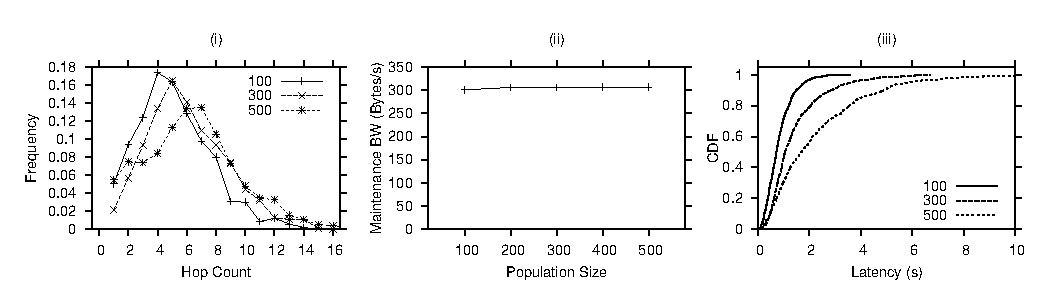
\includegraphics{results/newgraphs/nochurn/nochurn}}
\caption{Performance of static Chord networks of different sizes.
(i) shows hop-count distribution for lookups, (ii)
shows maintenance traffic in the absence of churn for
different population sizes; and (iii)
shows measured cumulative distribution of the latency over all lookups.}
\label{fig:static}
\end{figure*}

% % % % % % % % % % % % % % % % % % % % % % % % % % % % % % % % % % 
\section{Evaluation}
\label{sec:evaluation}
In this section we present performance results from \Sys.  We have two
goals 
in this evaluation.  First, we wish to validate that our simple
declarative specifications of complex overlays result in the expected
network properties, including topological properties and messaging
overheads.  Second, we examine our raw performance with an eye toward
feasibility: we do not expect our per-node performance to be as
good as a highly-tuned hand-coded implementation, but we would like it to be 
acceptable.

In our experiments, we focus on the full Chord DHT specification
in Appendix~\ref{sec:chordOverlog}.  
We chose to present Chord results largely because it is a good stress
test of our architecture, being relatively complex compared to other
examples like gossip and end-system multicast.  Chord also has the
advantage of being well-studied. 

We deployed \Sys on the Emulab testbed~\cite{White+:osdi02},
with instances of \Sys spread over a
network of 100 machines.  Except where noted, the network is a
GT-ITM transit-stub topology with 10 transit domains and 100 stubs
(one per physical node) emulated using DummyNet on 10 additional
machines. The RTT between two transit nodes is 50ms, while the RTT
between two nodes in the same domain is 2ms. The link capacity is set to
100Mbps and 10Mbps for domain and stub nodes respectively.

\subsection{Feasibility Experiments}
We begin with the
high-level characteristics of the Chord overlay, to validate that the \Sys
implementation exhibits the expected properties. We generate
a uniform workload of DHT ``lookup'' requests to a static membership
of nodes in the overlay, with no nodes joining or leaving.  This is
somewhat unrealistic but it allows us to observe the static properties
of Chord.

Figure~\ref{fig:static}(i) shows the hop-count distribution for our
workload.  As expected, the 
hop-count averages $\log N/2$, where $N$ is the size of the network.
Figure~\ref{fig:static}(ii) shows the maintenance traffic for the
network; this is the bandwidth used by the nodes while idling.  As can
be seen, our overlay is configured to use relatively low bandwidth --
networks aiming at high consistency and low latency typically use
about 1 KByte/s per node~\cite{rhea_usenix_2004}. 

Figure~\ref{fig:static}(iii) shows the raw latency performance of our
implementation.  While the latency increases with network size
(as might be expected), on a 500-node static network 96\% of all lookups 
complete in 6 seconds or less. Our latency numbers are within the same
order of magnitude as the published numbers~\cite{chord} of the MIT Chord deployment.

\subsection{Handling Churn}
In our second round of experiments, we focus on the performance of our
Chord implementation under varying degrees of membership churn.
Again, our goal is to validate that our compact specification of Chord
faithfully captures its salient properties.   We bring up a 400 node
Chord network, and then churn the network for 20 minutes, following
the methodology in~\cite{rhea_usenix_2004}.   

\begin{figure*}[t]
\centerline{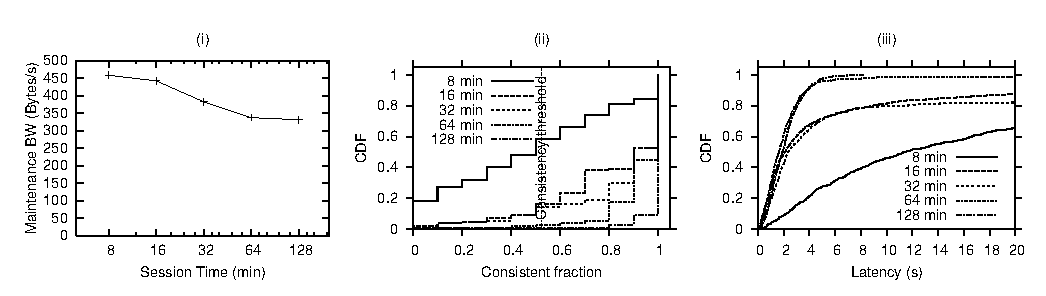
\includegraphics{results/newgraphs/churn/churn}}
\caption{Performance of a 400-node Chord overlay under varying
degrees of churn (8, 16, 32, 64, and 128 minute session times).
(i) shows maintenance traffic over time during our
experiment; (ii) shows consistency of lookups
over time, and (iii) shows lookup
latency under churn.  Each is a
cumulative distribution over all lookups. }
\label{fig:churn}
\end{figure*}

Figure~\ref{fig:churn} shows our results.  The
first graph (i) measures the ``maintenance traffic'' for the network,
that is, all traffic not associated with lookups and responses.  This
includes traffic for checking the status of nodes in the network, and
recovery traffic as the nodes come and go.  As in the static case, our
maintenance traffic is fairly respectable.

Figure~\ref{fig:churn}(ii) examines consistency of lookups
(following the experimental setup of Bamboo~\cite{rhea_usenix_2004}),
and Figure~\ref{fig:churn}(iii)
considers raw latency of external (i.e., non-maintenance-related) lookups
under churn. \Sys Chord does respectably under low churn (session times
of 64 minutes and above), generating at least 97\% consistent
lookups, most of which complete within 4 seconds. On the other hand,
under high churn (session times of 16 minutes and less), \Sys Chord does not
perform well, producing only 42\% and 84\% consistent lookups with high latencies.

Ultimately, an evaluation of a system like \Sys rests on an assessment
of the ideal tradeoff between code size and performance.  Our current
Chord overlay written in \Lang performs acceptably, but clearly does not
attain the published figures for the MIT implementation (at least 99.9\%
consistency for a session time of 47 minutes, and mean lookup latency of
less than 5 seconds under high churn). 

We conjecture that a carefully crafted and complete MACEDON
implementation of Chord might outperform our \PChordLines 
\Lang rules, but it would be more than an order of magnitude more complex.  
We note that the 320-line version supplied with the 
distribution\footnote{See \texttt{chord.mac} in MACEDON release
1.2.1-20050531, from \url{http://macedon.ucsd.edu/release/}.}
is not sufficiently complete to evaluate under churn or compare
meaningfully to MIT Chord or our implementation over P2; for example,
MACEDON's Chord implements 32-bit node identifiers instead of the
traditional 160 bits, and provides only a single successor for each
node, making it highly likely that the ring becomes partitioned.


% % % % % % % % % % % % % % % % % % % % % % % % % % % % % % % % % % 
\section{Related work}
\label{sec:related}
The design of \Sys can be viewed as a synthesis of ideas from database
systems, particularly recent work in distributed and continuous query
processing, with logic languages, and the result applied to overlay
networks.   Throughout this paper we have highlighted the database
systems techniques we have employed in \Sys; in this section we
situate \Lang and \Sys's approach in the context of existing work on
generating overlays from protocol descriptions. 

There is a long tradition of automating the generation of protocol
implementations from specifications.  Much of the early work focuses
on expressing OSI protocols in a finite state machine language
(Esterel, Estelle, LOTOS, SDL~\cite{esterel,fdt-book}, etc.), and
compiling them into CPU-efficient implementations
(e.g., \cite{dabbous-sigcomm96,vuong-estelle-tose88}).  The focus of
this body of work is on supporting formal protocol specification
(e.g., for verification), ideally without sacrificing CPU performance.

More recently, there has been increased emphasis on readability and
code reuse for network protocol specification languages.  This
includes domain-specific object-oriented languages like
Morpheus~\cite{morpheus} and Prolac~\cite{prolac}, and functional
approaches like the Fox project's TCP implementation~\cite{fox}.

It is typical to think of implementing network protocols in terms of
state machines, whose transitions are triggered by timer events or the
arrival of messages (either over the network or from a local client
application).  This is the approach taken in essentially all of the
work cited above.  Network protocol stacks are typically implemented
in such a manner even when hand-coded, and this approach lends itself
to object-oriented programming languages, where finite state machines (FSMs) are encapsulated
in software objects.  

Overlays built using an FSM approach are generally event-driven from a
Unix ``select'' loop or equivalent OS functionality, and can be highly
efficient in terms of resource usage (CPU, etc.) on a node.  A recent
example of this approach is MACEDON~\cite{rodriguez04macedon}, which
adopts the FSM approach by
encapsulating the event loop, timers, finite state 
machines, and message formats, and compiling the resulting syntactic
elements to C++.   Because the output of the MACEDON compiler closely
mirrors the structure of the code that a skilled programmer would
produce for an overlay, we believe that the performance of a
well-tuned MACEDON network could approach a custom implementation with
less code than C++ would require, though the current MACEDON overlay
suite does not approach this. 

An interesting alternative to state machines is
RTAG~\cite{anderson88rtag}, 
where the protocol is expressed as a grammar.  Incoming messages and
events are modeled as tokens causing reductions in grammar rules, and
the state of a connection is held on the parser stack rather than
encapsulated in an FSM.  

The $i3$~\cite{i3} infrastructure offers a rendezvous-based
abstraction that provides significant flexibility in specifying
communication structures and patterns.  $i3$ is similar in fundamental
ways to the relational abstraction used in \Sys -- the decoupling of
senders and receivers via keys in $i3$ is similar to the keys and
foreign keys of relational models, and the same flexible indirections
are possible in both.  However, $i3$ is targeted as a fundamental
communication abstraction, whereas \Sys is a more functional but
arguably more special-purpose system.

Although Click's configuration language unambiguously specifies the
dataflow elements and graph to be generated, the idea of using a
high-level logic language for describing network protocols seems
relatively new.  Loo et al.~\cite{loo-hotnets04} recently proposed
performing IP routing using declarative queries, also written in a
variant of Datalog.  Our implementation of \Sys is focused on overlay
construction rather than IP routing, but as we discussed in
Section~\ref{sec:planner}, some of the optimization techniques
suggested in~\cite{loo-hotnets04} from the deductive database
literature are applicable in \Sys. 

As in~\cite{loo-hotnets04}, by representing the desired
network properties in \Lang at a higher level of abstraction than a
dataflow graph, protocol grammar, or FSM description, \Sys achieves
very concise 
descriptions that can nevertheless generate executable dataflow graphs 
to maintain the overlay. 

In addition to conciseness, as section~\ref{sec:overlog} discusses, a
top-down approach like \Lang offers more opportunities for compile- and
run-time optimization of overlay descriptions, and \Lang's
decomposition of state into tables and flows provides more natural
opportunities for code reuse and runtime sharing.  


% % % % % % % % % % % % % % % % % % % % % % % % % % % % % % % % % % 
\section{Conclusion and Future Work}
\label{sec:conclusion}

In this paper, we have investigated the feasibility of expressing
overlay networks in a declarative language, and then directly
executing the resulting specification to construct and maintain the
overlay network.  

The approach looks promising: overlays can be specified extremely
concisely, yet with enough detail to be executed with performance and
robustness acceptable for many applications.   Furthermore, \Lang
makes it easy to alter overlay routing algorithms without
reimplementing complex state machines.

Our current system successfully compiles and runs
specifications for all overlays discussed in this
paper.  Our planner does not currently handle
directly some of the more involved constructs of
the \Lang language, such as multi-node rule bodies
and the logic of negation; slightly wordier rule rewrites allow us
to circumvent these limitations, as the next
design iteration of the planner takes shape.  The
appendices contain overlay specifications
that are executable by our system as of July 2005.

We continue our efforts in several directions.

{\bf Breadth:} In the short term, we
are working on coding a variety 
of other overlay networks in \Lang: epidemic-based networks,
link-state- and path-vector-based overlays, and further DHT schemes.
This has the benefit of exercising the 
\Sys planner and ensuring that \Lang is sufficiently expressive to
cover the design space, but will also enable us to start to identify
common constructs that can be factored out of particular overlay
specifications and shared. 

{\bf Sharing:} Sharing is intriguing
not only in terms of code reuse, but also for the
possibility that multiple overlays can execute
simultaneously, sharing state, communication, and
computation by sharing dataflow subgraphs.  Sharing
between multiple overlays can allow a single
application to achieve different performance goals
for different tasks, by efficiently deploying
multiple overlay variants simultaneously.  For
example, a peer-to-peer content distribution
network that combines search with parallel download
might choose to construct two different overlays
for these very different tasks.  These overlays
might fruitfully share rules for liveness checking,
latency and bandwidth estimation, etc.  Runtime
sharing across overlays can also allow
separately deployed systems to co-exist efficiently
within a shared network infrastructure; 
this might become important if overlays emerge as a
prevalent usage model for the Internet.

The na\"{i}ve approach for sharing is to do so explicitly at the \Lang
level, by sharing rule specifications.  However, we hope to
apply multiquery optimization techniques from the database literature
to identify further sharing opportunities automatically, within
the \Sys planner.  This enhancement to the planner will be in tandem
with applying some of the single query optimization techniques we
mentioned in section~\ref{sec:planner}.


{\bf Transport Protocols:} While bringing different
overlays to \Sys, we have rediscovered the
multifaceted nature of overlay requirements on
network and transport facilities.  Different
applications require different combinations of
reliable, in-order, congestion-, and
flow-controlled transports, and different levels of
control and inspection for each.  For example,
going from applying TCP-friendly congestion control
on a per-peer basis (as in
Bamboo~\cite{rhea_usenix_2004}) to having a single
congestion window for the whole node (as in MIT
Chord~\cite{li04comparing}) is a matter of design
requirements that may not be sufficiently addressed
by a monolithic transport solution.  \Sys's
dataflow architecture makes such choices as simple
as rearranging the bindings between a few common
elements.

Similarly, making the transport ``layer'' a graph
of dataflow elements means that different bits of
functionality can be broken up and spread out
throughout the application logic.  For instance,
one can push transmission retries to happen
upstream of route selection, to allow nodes route
flexibility when the next hop is not the ultimate
destination for a transmission.  Or, an application
can push a transmit buffer upstream, near where
tuples are first produced, reducing the amount of
queuing that tuples encounter outside of \Sys,
which minimizes the time during which they are
unavailable for computation.  Instead, tuples are
available for computation as soon as possible after
they arrive on a node, getting pulled out of a
table, routed, marshaled, and sent only when the
corresponding socket can send data, the congestion
window has room, and the outgoing packet scheduler
has selected the tuple's dataflow.


{\bf On-line distributed debugging:} A unique
opportunity offered by our system is its
\emph{multi-resolution} programming paradigm, allowing
the programmer to specify a system as a set of
logical rules, which are translated to a dataflow
graph and then executed at runtime.  By
exposing the execution history of the system -- in
terms of rules that fired at a first level, or in
terms of actions taken by each dataflow element at
a second level -- \Sys is astonishingly capable to
provide introspection support for on-line overlay
debugging.  In fact, since execution history at any
resolution can be exported as a set of relational
tables, much as everything else with \Sys,
debugging itself becomes an exercise in writing
\Lang rules for high-level invariants or for
execution history mining.  We are actively building
up the infrastructure within \Sys to 
evaluate the exciting debugging possibilities
that such support would enable.


{\bf Security:} It is a natural, short step (though perhaps
a precarious one) to move from system introspection
to security assessment.  \Sys's runtime composition
of small, simple dataflow elements along
with flat state tables implies that we might be
able to express security invariants for each
element in isolation, which would ideally compose
into global security properties for the whole
system.  We are exploring the application of our earlier work
on preserving the \emph{historic integrity} of a
distributed system~\cite{Maniatis2003thesis} to the
problem of making the execution of a complex
overlay \emph{tamper-evident}.


{\bf Language:} The version of \Lang that we
describe in this work is a strawman vehicle,
expressive enough to aid us in our initial exploration of
the design space.  We have produced a preliminary
formal semantics for \Lang, to enable reasoning
about program properties (safety, termination,
etc.).  We are also exploring the extensions in the
language that would permit a high-level
specification of sharing, transport, debugging, and security
logic, as described above.

We expect to revisit the choice of Datalog as a
basis for \Lang.  As we have discussed, Datalog's
generality makes it an ideal choice as a ``first
cut'' declarative language for overlays.  How \Lang
can be improved by tailoring its syntax and
semantics more specifically towards overlay
description is an interesting research direction.





\section{Acknowledgments}
We would like to thank our shepherd Dahlia Malkhi, Brent Chun for initial
encouragement and help using 
his distributed automated testing tool for our evaluation,
David Gay for his significant contributions to \Lang's operational
semantics, and Tristan Koo for testing code and performance
microbenchmarks.  We are also indebted to Brent, David, Ryan Huebsch,
Kevin Lai, Raghu Ramakrishnan, Sylvia Ratnasamy, and Sean Rhea, for
their thoughtful comments on drafts of this paper. Finally, our paper
has benefitted significantly from the detailed feedback offered by the
anonymous reviewers. 

{\small
%%\bibliography{paper}
\begin{thebibliography}{10}

\vskip 12pt

\bibitem{morpheus}
M.~B. Abbott and L.~L. Peterson.
\newblock A language-based approach to protocol implementation.
\newblock {\em IEEE/ACM Transactions on Networking}, 1(1), Feb. 1993.

\bibitem{alicebook}
S.~Abiteboul, R.~Hull, and V.~Vianu.
\newblock {\em Foundations of Databases}.
\newblock Addison Wesley, 1995.

\bibitem{anderson88rtag}
D.~P. Anderson.
\newblock Automated protocol implementation with {RTAG}.
\newblock {\em IEEE Trans. Softw. Eng.}, 14(3):291--300, 1988.

\bibitem{aurora}
H.~Balakrishnan, M.~Balazinska, D.~Carney, U.~Cetintemel, M.~Cherniack,
  C.~Convey, E.~Galvez, J.~Salz, M.~Stonebraker, N.~Tatbul, R.~Tibbetts, and
  S.~Zdonik.
\newblock Retrospective on {A}urora.
\newblock {\em VLDB Journal}, 13(4), Dec. 2004.

\bibitem{esterel}
G.~Berry.
\newblock {\em The Foundations of Esterel}, pages 425--454.
\newblock MIT Press, 1998.

\bibitem{fox}
E.~Biagioni.
\newblock A structured {TCP} in {S}tandard {ML}.
\newblock In {\em Proc. SIGCOMM}, 1994.

\bibitem{telegraphcq}
S.~Chandrasekaran, O.~Cooper, A.~Deshpande, M.~J. Franklin, J.~M. Hellerstein,
  W.~Hong, S.~Krishnamurthy, S.~Madden, V.~Raman, F.~Reiss, and M.~A. Shah.
\newblock {TelegraphCQ}: Continuous dataflow processing for an uncertain world.
\newblock In {\em CIDR}, 2003.

\bibitem{chu00case}
Y.-H. Chu, S.~G. Rao, and H.~Zhang.
\newblock A case for end system multicast.
\newblock In {\em Proc. of ACM SIGMETRICS}, pages 1--12, 2000.

\bibitem{dabbous-sigcomm96}
W.~Dabbous, S.~W. O'Malley, and C.~Castelluccia.
\newblock Generating efficient protocol code from an abstract specification.
\newblock In {\em Proc. SIGCOMM}, pages 60--72, 1996.

\bibitem{dabek_nsdi04}
F.~Dabek, J.~Li, E.~Sit, F.~Kaashoek, R.~Morris, and C.~Blake.
\newblock Designing a {DHT} for low latency and high throughput.
\newblock In {\em Proc. NSDI}, Month 2004.

\bibitem{dvmrp}
S.~Deering and D.~R. Cheriton.
\newblock Multicast routing in datagram internetworks and extended {LAN}s.
\newblock {\em ACM Transactions on Computer Systems}, 8(2):85--111, May 1990.

\bibitem{gamma}
D.~J. DeWitt, R.~H. Gerber, G.~Graefe, M.~L. Heytens, K.~B. Kumar, and
  M.~Muralikrishna.
\newblock Gamma - a high performance dataflow database machine.
\newblock In {\em VLDB}, pages 228--237, 1986.

\bibitem{estelle-success}
M.~Fecko, M.~Uyar, P.~Amer, A.~Sethi, T.~Dzik, R.~Menell, and M.~McMahon.
\newblock A success story of formal description techniques: Estelle
  specification and test generation for {MIL-STD 188-220}.
\newblock {\em Computer Communications (Special Edition on FDTs in Practice)},
  23, 2000.

\bibitem{graefe-sigmod90}
G.~Graefe.
\newblock Encapsulation of parallelism in the {V}olcano query processing
  system.
\newblock In {\em Proc. of the 1990 ACM SIGMOD International Conference on
  Management of Data, Atlantic City, NJ, May 23-25, 1990}, pages 102--111. ACM
  Press, 1990.

\bibitem{handley05xorp}
M.~Handley, A.~Ghosh, P.~Radoslavov, O.~Hodson, and E.~Kohler.
\newblock Designing extensible {IP} router software.
\newblock In {\em Proc. NSDI}, May 2005.

\bibitem{pier-cidr}
R.~Huebsch, B.~N. Chun, J.~M. Hellerstein, B.~T. Loo, P.~Maniatis, T.~Roscoe,
  S.~Shenker, I.~Stoica, and A.~R. Yumerefendi.
\newblock The architecture of {PIER}: an {I}nternet-scale query processor.
\newblock In {\em CIDR}, pages 28--43, 2005.

\bibitem{prolac}
E.~Kohler, M.~F. Kaashoek, and D.~R. Montgomery.
\newblock A readable {TCP} in the {P}rolac protocol language.
\newblock In {\em Proc. SIGCOMM}, 1999.

\bibitem{click-tocs}
E.~Kohler, R.~Morris, B.~Chen, J.~Jannotti, and M.~F. Kaashoek.
\newblock The {C}lick modular router.
\newblock {\em ACM Trans. Comput. Syst.}, 18(3):263--297, 2000.

\bibitem{leighton-book}
F.~T. Leighton.
\newblock {\em Introduction to Parallel Algorithms and Architectures: Arrays,
  Trees, Hypercubes}.
\newblock Morgan Kaufmann, San Mateo, CA, 1992.

\bibitem{li04comparing}
J.~Li, J.~Stribling, T.~Gil, R.~Morris, and F.~Kaashoek.
\newblock Comparing the performance of distributed hash tables under churn.
\newblock In {\em Proc. IPTPS}, 2004.

\bibitem{loo-hotnets04}
B.~T. Loo, J.~M. Hellerstein, and I.~Stoica.
\newblock Customizable routing with declarative queries.
\newblock In {\em Third Workshop on Hot Topics in Networks (HotNets-III)}, Nov.
  2004.

\bibitem{Maniatis2003thesis}
P.~Maniatis.
\newblock {\em {Historic Integrity in Distributed Systems}}.
\newblock PhD thesis, Computer Science Department, Stanford University,
  Stanford, {CA}, {USA}, Aug. 2003.

\bibitem{symphony}
G.~Manku, M.~Bawa, and P.~Raghavan.
\newblock Symphony: Distributed hashing in a small world.
\newblock In {\em Proc. USITS}, 2003.

\bibitem{mazieres-usenix-2001}
D.~Mazi\`eres.
\newblock A toolkit for user-level file systems.
\newblock In {\em Proc. of the 2001 USENIX Technical Conference}, June 2001.

\bibitem{scout}
D.~Mosberger and L.~L. Peterson.
\newblock Making paths explicit in the {S}cout operating system.
\newblock In {\em Proc. OSDI}, pages 153--167. ACM Press, 1996.

\bibitem{stream}
R.~Motwani, J.~Widom, A.~Arasu, B.~Babcock, S.~Babu, M.~Datar, G.~S. Manku,
  C.~Olston, J.~Rosenstein, and R.~Varma.
\newblock Query processing, approximation, and resource management in a data
  stream management system.
\newblock In {\em Proc. CIDR}, 2003.

\bibitem{monsoon}
G.~M. Papadopoulos and D.~E. Culler.
\newblock Monsoon: An explicit token store architecture.
\newblock In {\em Proc. ISCA}, May 1990.

\bibitem{shankar-stems}
V.~Raman, A.~Deshpande, and J.~M. Hellerstein.
\newblock Using state modules for adaptive query processing.
\newblock In {\em Proc. ICDE}, 2003.

\bibitem{rhea_usenix_2004}
S.~Rhea, D.~Geels, T.~Roscoe, and J.~Kubiatowicz.
\newblock Handling {C}hurn in a {DHT}.
\newblock In {\em Proc. of the 2004 USENIX Technical Conference, Boston, MA,
  USA}, June 2004.

\bibitem{rodriguez04macedon}
A.~Rodriguez, C.~Killian, S.~Bhat, D.~Kostic, and A.~Vahdat.
\newblock {MACEDON}: {M}ethodology for {A}utomatically {C}reating,
  {E}valuating, and {D}esigning {O}verlay {N}etworks",.
\newblock In {\em Proc. NSDI}, March 2004.

\bibitem{selinger79}
P.~G. Selinger, M.~M. Astrahan, D.~D. Chamberlin, R.~A. Lorie, and T.~G. Price.
\newblock Access path selection in a relational database management system.
\newblock In {\em SIGMOD Conference}, pages 23--34, 1979.

\bibitem{sellis-mqo}
T.~Sellis.
\newblock {Multiple Query Optimization}.
\newblock {\em ACM Transactions on Database Systems}, 13(1):23--52, Mar. 1988.

\bibitem{i3}
I.~Stoica, D.~Adkins, S.~Zhaung, S.~Shenker, and S.~Surana.
\newblock Internet indirection infrastructure.
\newblock {\em IEEE/ACM Transactions on Networking}, (2), Apr. 2004.

\bibitem{chord}
I.~Stoica, R.~Morris, D.~Liben-Nowell, D.~R. Karger, M.~F. Kaashoek, F.~Dabek,
  and H.~Balakrishnan.
\newblock Chord: a scalable peer-to-peer lookup protocol for internet
  applications.
\newblock {\em IEEE/ACM Trans. Netw.}, 11(1):17--32, 2003.

\bibitem{fdt-book}
K.~J. Turner, editor.
\newblock {\em Using formal description techniques -- An Introduction to
  {E}stelle, {LOTOS} and {SDL}}.
\newblock Wiley, 1993.

\bibitem{dataflowarch}
A.~H. Veen.
\newblock Dataflow machine architecture.
\newblock {\em ACM Computing Surveys}, 18(4), Dec. 1986.

\bibitem{vuong-estelle-tose88}
S.~T. Vuong, A.~C. Lau, and R.~I. Chan.
\newblock Semiautomatic implementation of protocols using an {E}stelle-{C}
  compiler.
\newblock {\em IEEE Transactions on Software Engineering}, 14(3), Mar. 1988.

\bibitem{White+:osdi02}
B.~White, J.~Lepreau, L.~Stoller, R.~Ricci, S.~Guruprasad, M.~Newbold,
  M.~Hibler, C.~Barb, and A.~Joglekar.
\newblock An integrated experimental environment for distributed systems and
  networks.
\newblock In {\em Proc.\ OSDI 2002}, Boston, MA, Dec. 2002.

\end{thebibliography}

}
\newpage
\appendix

\section{Narada in \Lang}
\label{sec:naradaOverlog}

Here we provide an executable \Lang implementation of Narada's mesh
maintenance algorithms. Current limitations of the \Sys parser and
planner require slightly wordier syntax for some of our 
constructs.  Specifically, handling of negation is still incomplete,
requiring that we rewrite some rules to eliminate negation.
Furthermore, our planner currently handles rules with collocated terms
only.  The \Lang specification below is directly parsed and executed by our
current codebase.

\begin{overlog}
/** Base tables */

materialize(member, infinity, infinity, keys(2)).
materialize(sequence, infinity, 1, keys(2)).
materialize(neighbor, infinity, infinity, keys(2)).


/* Environment table containing configuration
   values */

materialize(env, infinity, infinity, keys(2,3)).


/* Setup of configuration values */

E0 neighbor@X(X,Y) :- periodic@X(X,E,0,1), env@X(X,
  H, Y), H == "neighbor".


/** Start with sequence number 0 */

S0 sequence@X(X, Sequence) :- periodic@X(X, E, 0,
  1), Sequence := 0.


/** Periodically start a refresh */

R1 refreshEvent@X(X) :- periodic@X(X, E, 3).


/** Increment my own sequence number */

R2 refreshSequence@X(X, NewSequence) :-
  refreshEvent@X(X), sequence@X(X, Sequence),
  NewSequence := Sequence + 1.


/** Save my incremented sequence */

R3 sequence@X(X, NewSequence) :-
  refreshSequence@X(X, NewSequence).


/** Send a refresh to all neighbors with my current
  membership */

R4 refresh@Y(Y, X, NewSequence, Address, ASequence,
  ALive) :- refreshSequence@X(X, NewSequence),
  member@X(X, Address, ASequence, Time, ALive),
  neighbor@X(X, Y).


/** How many member entries that match the member
  in a refresh message (but not myself) do I have? */

R5 membersFound@X(X, Address, ASeq, ALive,
  count<*>) :- refresh@X(X, Y, YSeq, Address, ASeq,
  ALive), member@X(X, Address, MySeq, MyTime,
  MyLive), X != Address.


/** If I have none, just store what I got */

R6 member@X(X, Address, ASequence, T, ALive) :-
  membersFound@X(X, Address, ASequence, ALive, C),
  C == 0, T := f_now().


/** If I have some, just update with the
  information I received if it has a higher
  sequence number. */

R7 member@X(X, Address, ASequence, T, ALive) :-
  membersFound@X(X, Address, ASequence, ALive, C),
  C > 0, T := f_now(), member@X(X, Address,
  MySequence, MyT, MyLive), MySequence < ASequence.


/** Update my neighbor's member entry */

R8 member@X(X, Y, YSeq, T, YLive) :- refresh@X(X,
  Y, YSeq, A, AS, AL), T := f_now(), YLive := 1.


/** Add anyone from whom I receive a refresh
  message to my neighbors */

N1 neighbor@X(X, Y) :- refresh@X(X, Y,
  YS, A, AS, L).


/** Probing of neighbor liveness */

L1 neighborProbe@X(X) :- periodic@X(X, E, 1).
L2 deadNeighbor@X(X, Y) :- neighborProbe@X(X), T :=
  f_now(), neighbor@X(X, Y), member@X(X, Y, YS, YT,
  L), T - YT > 20.
L3 delete neighbor@X(X, Y) :- deadNeighbor@X(X, Y).
L4 member@X(X, Neighbor, DeadSequence, T, Live) :-
  deadNeighbor@X(X, Neighbor), member@X(X,
  Neighbor, S, T1, L), Live := 0, DeadSequence := S
  + 1, T:= f_now().
\end{overlog}



\section{Chord in \Lang}
\label{sec:chordOverlog}

Here we provide the full \Lang specification for Chord. This
specification deals with lookups, ring maintenance with a fixed number
of successors, finger-table maintenance and opportunistic finger table
population, joins, stabilization, and node failure detection.

\begin{overlog}
/* The base tuples */

materialize(node, infinity, 1, keys(1)).
materialize(finger, 180, 160, keys(2)).
materialize(bestSucc, infinity, 1, keys(1)).
materialize(succDist, 10, 100, keys(2)).
materialize(succ, 10, 100, keys(2)).
materialize(pred, infinity, 100, keys(1)).
materialize(succCount, infinity, 1, keys(1)).
materialize(join, 10, 5, keys(1)).
materialize(landmark, infinity, 1, keys(1)).
materialize(fFix, infinity, 160, keys(2)).  
materialize(nextFingerFix, infinity, 1, keys(1)).  
materialize(pingNode, 10, infinity, keys(2)).  
materialize(pendingPing, 10, infinity, keys(2)).  


/** Lookups */

L1 lookupResults@R(R,K,S,SI,E) :- node@NI(NI,N),
  lookup@NI(NI,K,R,E), bestSucc@NI(NI,S,SI), K in
  (N,S].
L2 bestLookupDist@NI(NI,K,R,E,min<D>) :-
  node@NI(NI,N), lookup@NI(NI,K,R,E),
  finger@NI(NI,I,B,BI), D:=K - B - 1, B in (N,K).
L3 lookup@BI(min<BI>,K,R,E) :- node@NI(NI,N),
  bestLookupDist@NI(NI,K,R,E,D),
  finger@NI(NI,I,B,BI), D == K - B - 1, B in (N,K).


/** Neighbor Selection */

N1 succEvent@NI(NI,S,SI) :- succ@NI(NI,S,SI).
N2 succDist@NI(NI,S,D) :- node@NI(NI,N),
  succEvent@NI(NI,S,SI), D:=S - N - 1.
N3 bestSuccDist@NI(NI,min<D>) :-
  succDist@NI(NI,S,D).
N4 bestSucc@NI(NI,S,SI) :- succ@NI(NI,S,SI),
  bestSuccDist@NI(NI,D), node@NI(NI,N), D == S - N
  - 1.
N5 finger@NI(NI,0,S,SI) :- bestSucc@NI(NI,S,SI).


/** Successor eviction */

S1 succCount@NI(NI,count<*>) :- succ@NI(NI,S,SI).
S2 evictSucc@NI(NI) :- succCount@NI(NI,C), C > 4.
S3 maxSuccDist@NI(NI,max<D>) :- succ@NI(NI,S,SI),
  node@NI(NI,N), evictSucc@NI(NI), D:=S - N - 1.
S4 delete succ@NI(NI,S,SI) :- node@NI(NI,N),
  succ@NI(NI,S,SI), maxSuccDist@NI(NI,D), D == S -
  N - 1.

/** Finger fixing */

F0 nextFingerFix@NI(NI, 0).
F1 fFix@NI(NI,E,I) :- periodic@NI(NI,E,10),
  nextFingerFix@NI(NI,I).
F2 fFixEvent@NI(NI,E,I) :- fFix@NI(NI,E,I).
F3 lookup@NI(NI,K,NI,E) :- fFixEvent@NI(NI,E,I),
  node@NI(NI,N), K:=1I << I + N.
F4 eagerFinger@NI(NI,I,B,BI) :- fFix@NI(NI,E,I),
  lookupResults@NI(NI,K,B,BI,E).
F5 finger@NI(NI,I,B,BI) :-
  eagerFinger@NI(NI,I,B,BI).
F6 eagerFinger@NI(NI,I,B,BI) :- node@NI(NI,N),
  eagerFinger@NI(NI,I1,B,BI), I:=I1 + 1, K:=1I << I
  + N, K in (N,B), BI != NI.
F7 delete fFix@NI(NI,E,I1) :-
  eagerFinger@NI(NI,I,B,BI), fFix@NI(NI,E,I1), I >
  0, I1 == I - 1.
F8 nextFingerFix@NI(NI,0) :-
  eagerFinger@NI(NI,I,B,BI), ((I == 159) || (BI ==
  NI)).
F9 nextFingerFix@NI(NI,I) :- node@NI(NI,N),
  eagerFinger@NI(NI,I1,B,BI), I:=I1 + 1, K:=1I << I
  + N, K in (B,N), NI != BI.


/** Churn Handling */

C1 joinEvent@NI(NI,E) :- join@NI(NI,E).
C2 joinReq@LI(LI,N,NI,E) :- joinEvent@NI(NI,E),
  node@NI(NI,N), landmark@NI(NI,LI), LI != "-".
C3 succ@NI(NI,N,NI) :- landmark@NI(NI,LI),
  joinEvent@NI(NI,E), node@NI(NI,N), LI == "-".
C4 lookup@LI(LI,N,NI,E) :- joinReq@LI(LI,N,NI,E).
C5 succ@NI(NI,S,SI) :- join@NI(NI,E),
  lookupResults@NI(NI,K,S,SI,E).


/** Stabilization */

SB0 pred@NI(NI,"-","-").
SB1 stabilize@NI(NI,E) :- periodic@NI(NI,E,15).
SB2 stabilizeRequest@SI(SI,NI) :-
  stabilize@NI(NI,E), bestSucc@NI(NI,S,SI).
SB3 sendPredecessor@PI1(PI1,P,PI) :-
  stabilizeRequest@NI(NI,PI1), pred@NI(NI,P,PI), PI
  != "-".
SB4 succ@NI(NI,P,PI) :- node@NI(NI,N),
  sendPredecessor@NI(NI,P,PI),
  bestSucc@NI(NI,S,SI), P in (N,S).
SB5 sendSuccessors@SI(SI,NI) :- stabilize@NI(NI,E),
  succ@NI(NI,S,SI).
SB6 returnSuccessor@PI(PI,S,SI) :-
  sendSuccessors@NI(NI,PI), succ@NI(NI,S,SI).
SB7 succ@NI(NI,S,SI) :-
  returnSuccessor@NI(NI,S,SI).
SB7 notifyPredecessor@SI(SI,N,NI) :-
  stabilize@NI(NI,E), node@NI(NI,N),
  succ@NI(NI,S,SI).
SB8 pred@NI(NI,P,PI) :- node@NI(NI,N),
  notifyPredecessor@NI(NI,P,PI),
  pred@NI(NI,P1,PI1), ((PI1 == "-") || (P in
  (P1,N))).


/** Connectivity Monitoring */

CM0 pingEvent@NI(NI,E) :- periodic@NI(NI,E,5).
CM1 pendingPing@NI(NI,PI,E) :- pingEvent@NI(NI,E),
  pingNode@NI(NI,PI).
CM2 pingReq@PI(PI,NI,E) :- pendingPing@NI(NI,PI,E).
CM3 delete pendingPing@NI(NI,PI,E) :-
  pingResp@NI(NI,PI,E).
CM4 pingResp@RI(RI,NI,E) :- pingReq@NI(NI,RI,E).
CM5 pingNode@NI(NI,SI) :- succ@NI(NI,S,SI), SI !=
  NI.
CM6 pingNode@NI(NI,PI) :- pred@NI(NI,P,PI), PI !=
  NI, PI != "-".
CM7 succ@NI(NI,S,SI) :- succ@NI(NI,S,SI),
  pingResp@NI(NI,SI,E).
CM8 pred@NI(NI,P,PI) :- pred@NI(NI,P,PI),
  pingResp@NI(NI,PI,E).
CM9 pred@NI(NI,"-","-") :- pingEvent@NI(NI,E),
  pendingPing@NI(NI,PI,E), pred@NI(NI,P,PI).

\end{overlog}


\end{document}

% LocalWords:  dataflow pseudocode multicast Datalog Prolog Narada refreshEvent
% LocalWords:  refreshSeq equijoins equijoin dataflows demultiplexer DHT
% LocalWords:  demultiplexed
